\documentclass[12pt]{article} % Sets the font size and document class

\usepackage[utf8]{inputenc} % Ensures encoding is set to UTF-8
\usepackage{graphicx} % Allows inclusion of images
\usepackage{geometry} % Adjusts the margins of the document
\usepackage{fancyhdr} % For custom headers and footers
\usepackage[croatian]{babel} 
\usepackage{amssymb}
\usepackage{amsmath}
\usepackage{txfonts}
\usepackage{mathdots}
\usepackage{titlesec}
\usepackage{array}
\usepackage{lastpage}
\usepackage{etoolbox}
\usepackage{tabularray}
\usepackage{color, colortbl}
\usepackage{adjustbox}
\usepackage{geometry}
\usepackage[classicReIm]{kpfonts}
\usepackage{hyperref}
\usepackage{fancyhdr}
\usepackage{advdate}
\usepackage{float}
\usepackage{setspace}
\restylefloat{table}

% Set page margins
\geometry{
	a4paper,
	left=25mm,
	right=25mm,
	top=30mm,
	bottom=30mm
}

% Set the header and footer style
\pagestyle{fancy}
\fancyhf{}
\rhead{Dominik Barukčić}
\lhead{LV6}
\rfoot{\thepage}

\title{LV6: Spajanje oblaka točaka postupkom iterativne najbliže točke}
\author{Dominik Barukčić}
\date{\today}

\begin{document}
	
	\maketitle
	
	\section{Uvod}
	Zadatak jest spojiti više oblaka točaka u jedinstveni
	oblak korištenjem postupka iterativne najbliže točke (ICP algoritam). Koristit ćemo dataset Garfield. Korišteni softver za izradu vježbe je MeshLab koji je dostupan na adresi https://www.meshlab.net.
	
	\section{Spajanje točaka}
	Otvorimo softver MeshLab. 
		\begin{figure}[H]
			\centering
			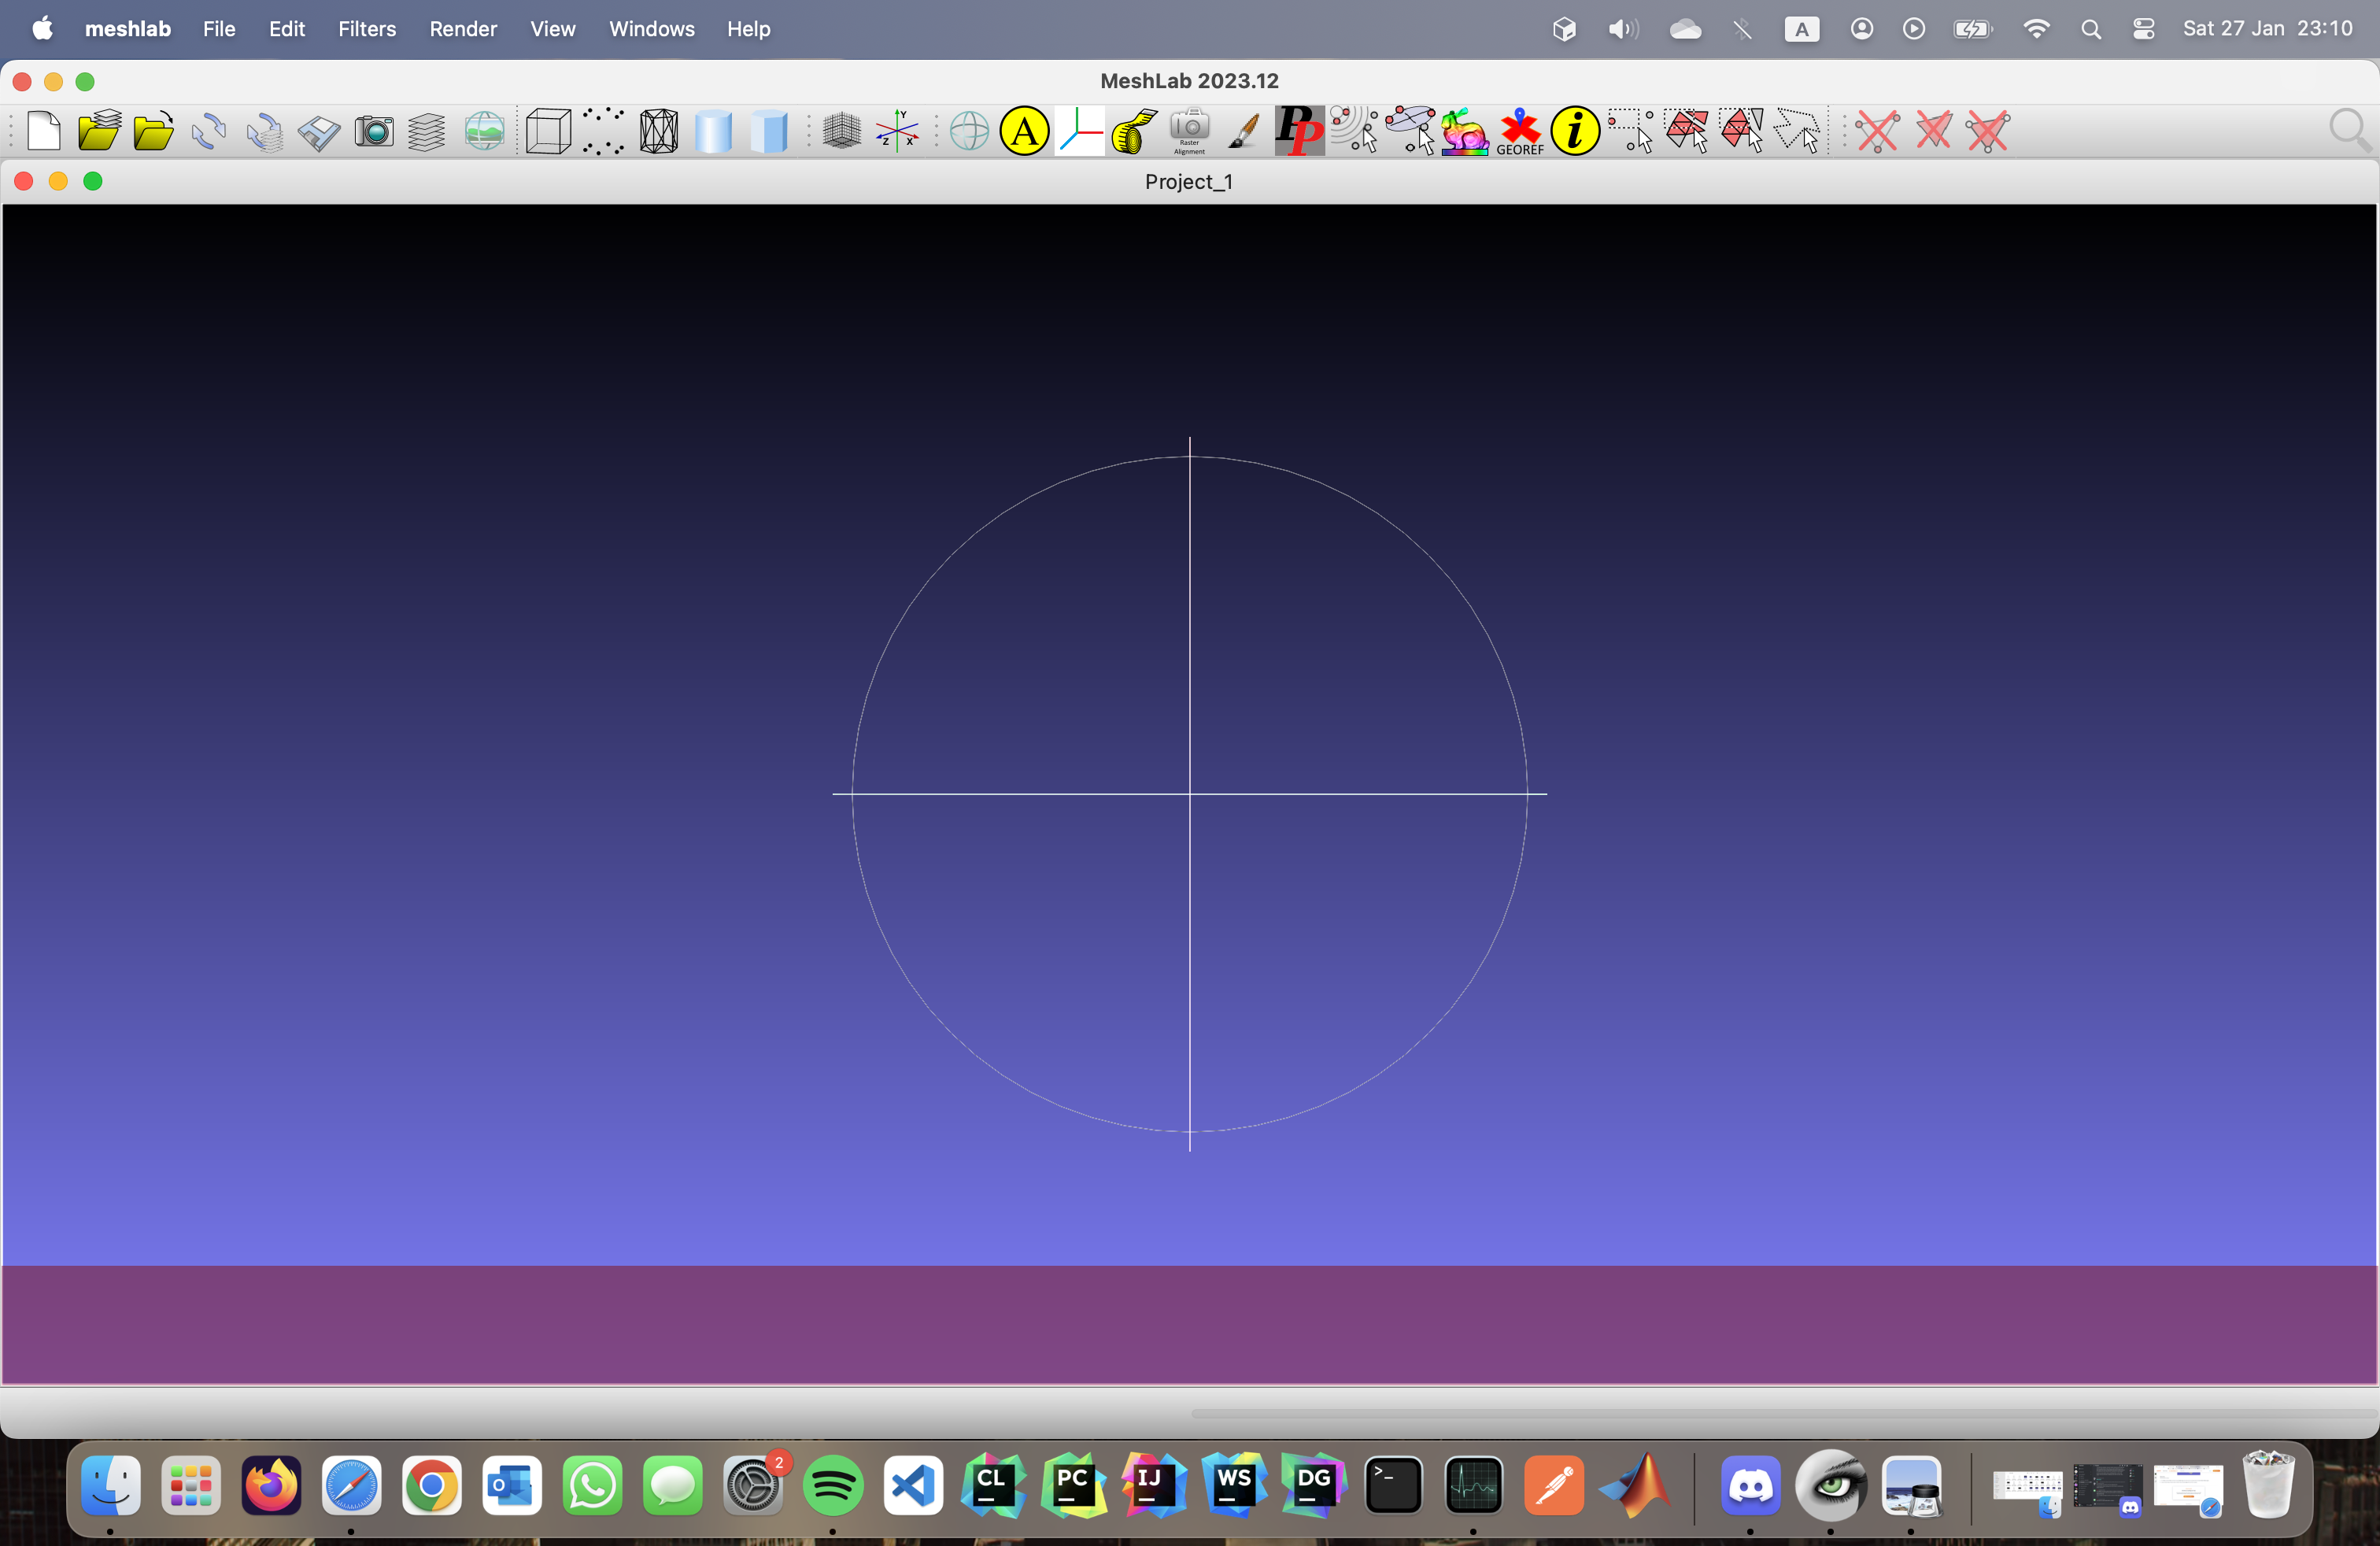
\includegraphics[width=1\textwidth]{screenshots/1.png}
			\caption{GUI MeshLab-a}
			\label{fig:yourlabel}
		\end{figure}
		
		Učitamo dataset Garfield.
		
		\begin{figure}[H]
			\centering
			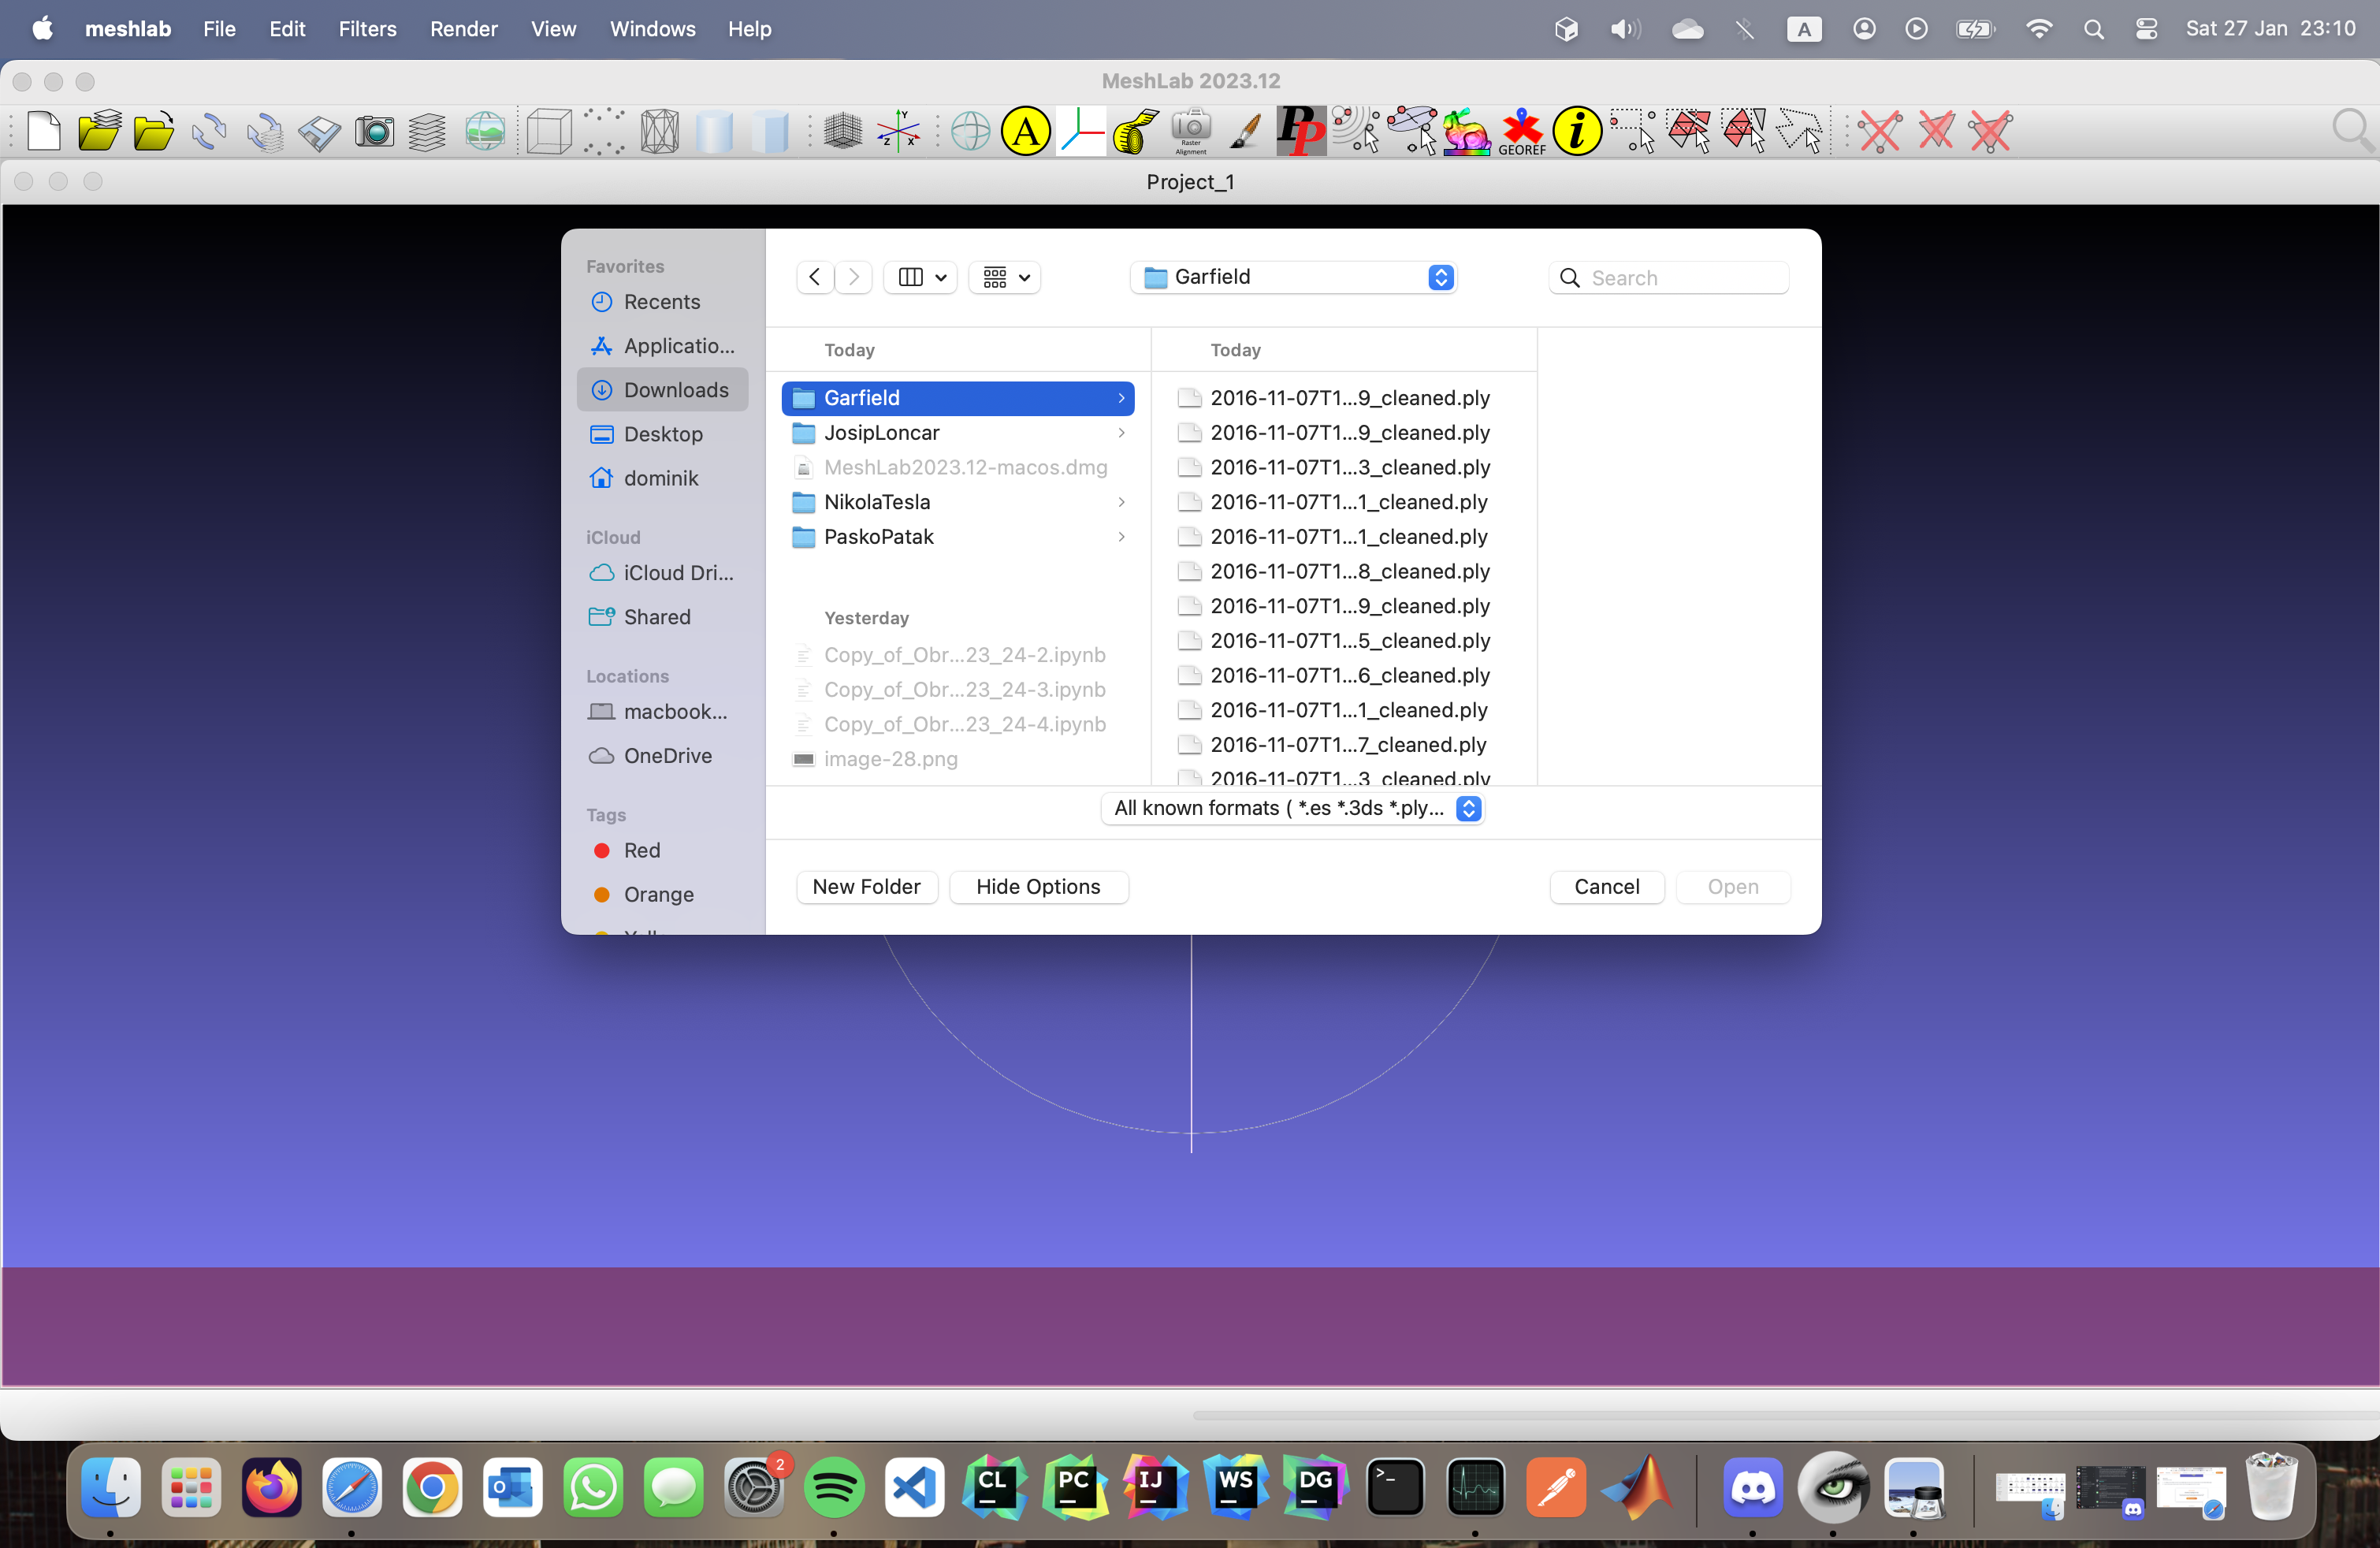
\includegraphics[width=1\textwidth]{screenshots/2.png}
			\caption{Prozor za dodavanje mesheva(.ply)}
			\label{fig:yourlabel}
		\end{figure}
		
		Moramo sad odznačiti sve mesheve, odnosno layere, kako ne bi bili vidljivi u 3D prostoru.
		\begin{figure}[H]
			\centering
			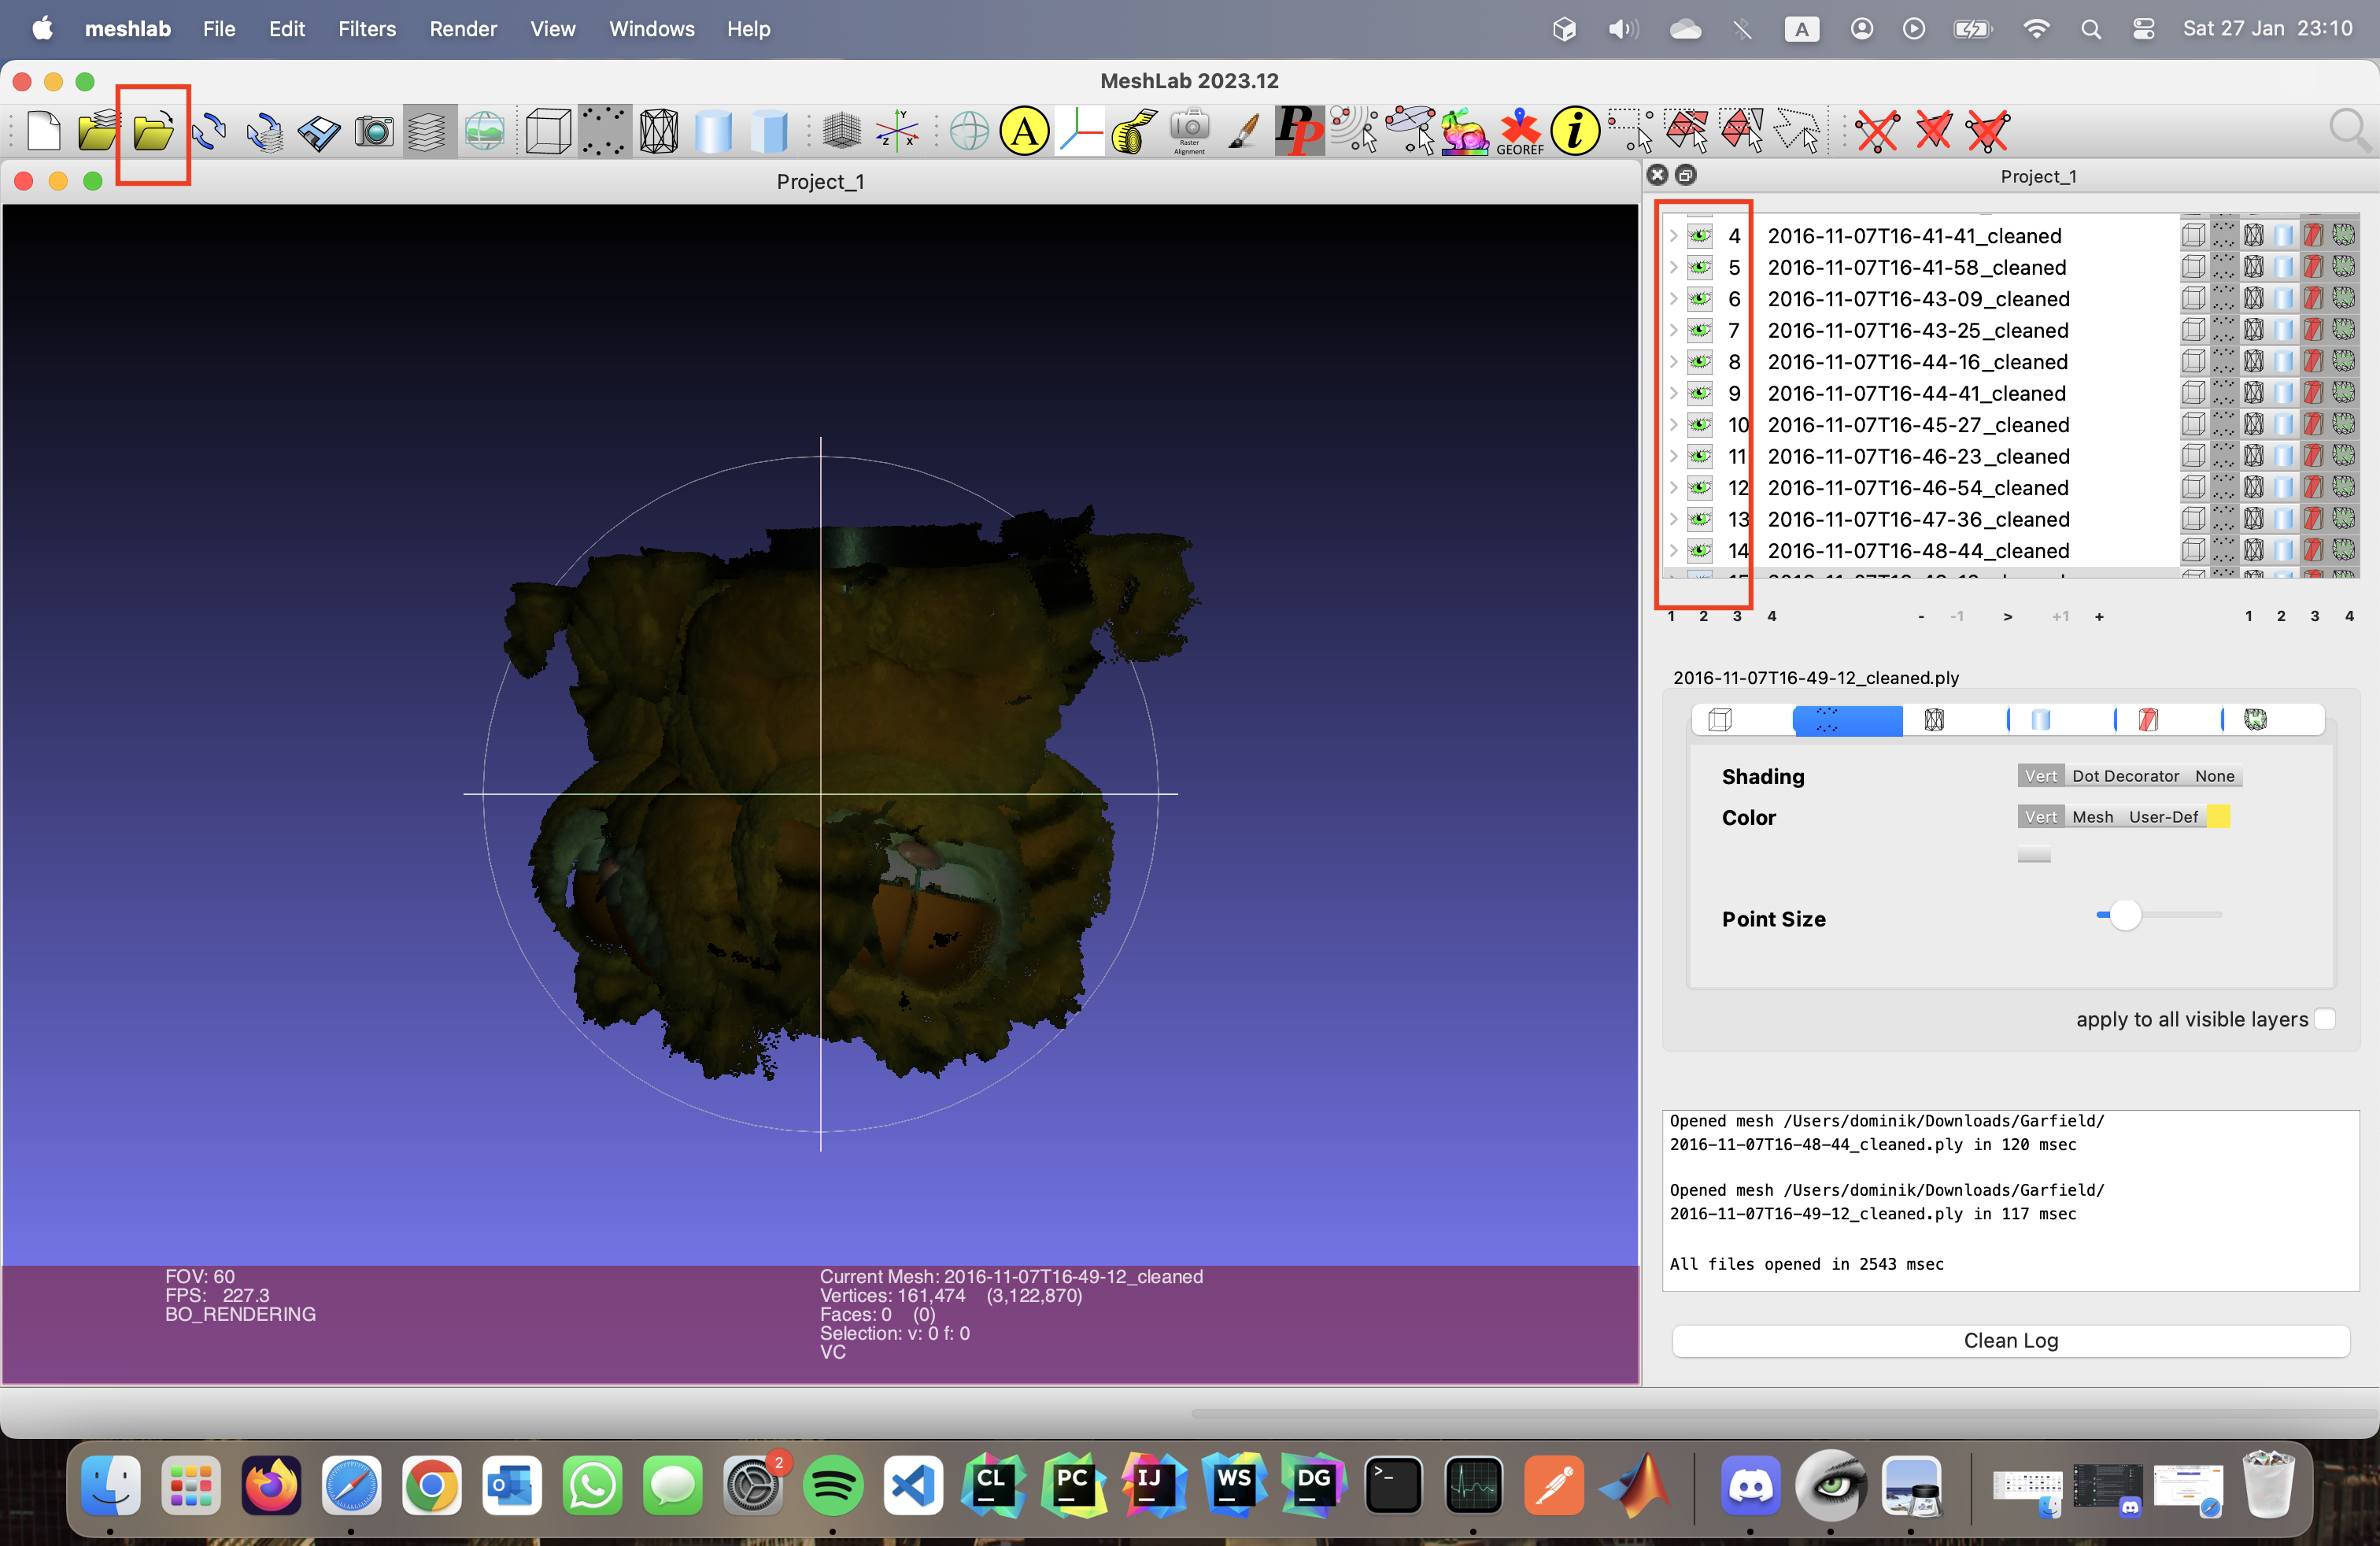
\includegraphics[width=0.5\textwidth]{screenshots/3.png}
			\caption{Prikazani su svi layeri}
			\label{fig:yourlabel}
		\end{figure}
		
		\pagebreak
		Označimo prvi layer i stisnemo Glue Mesh. 
		\begin{figure}[H]
			\centering
			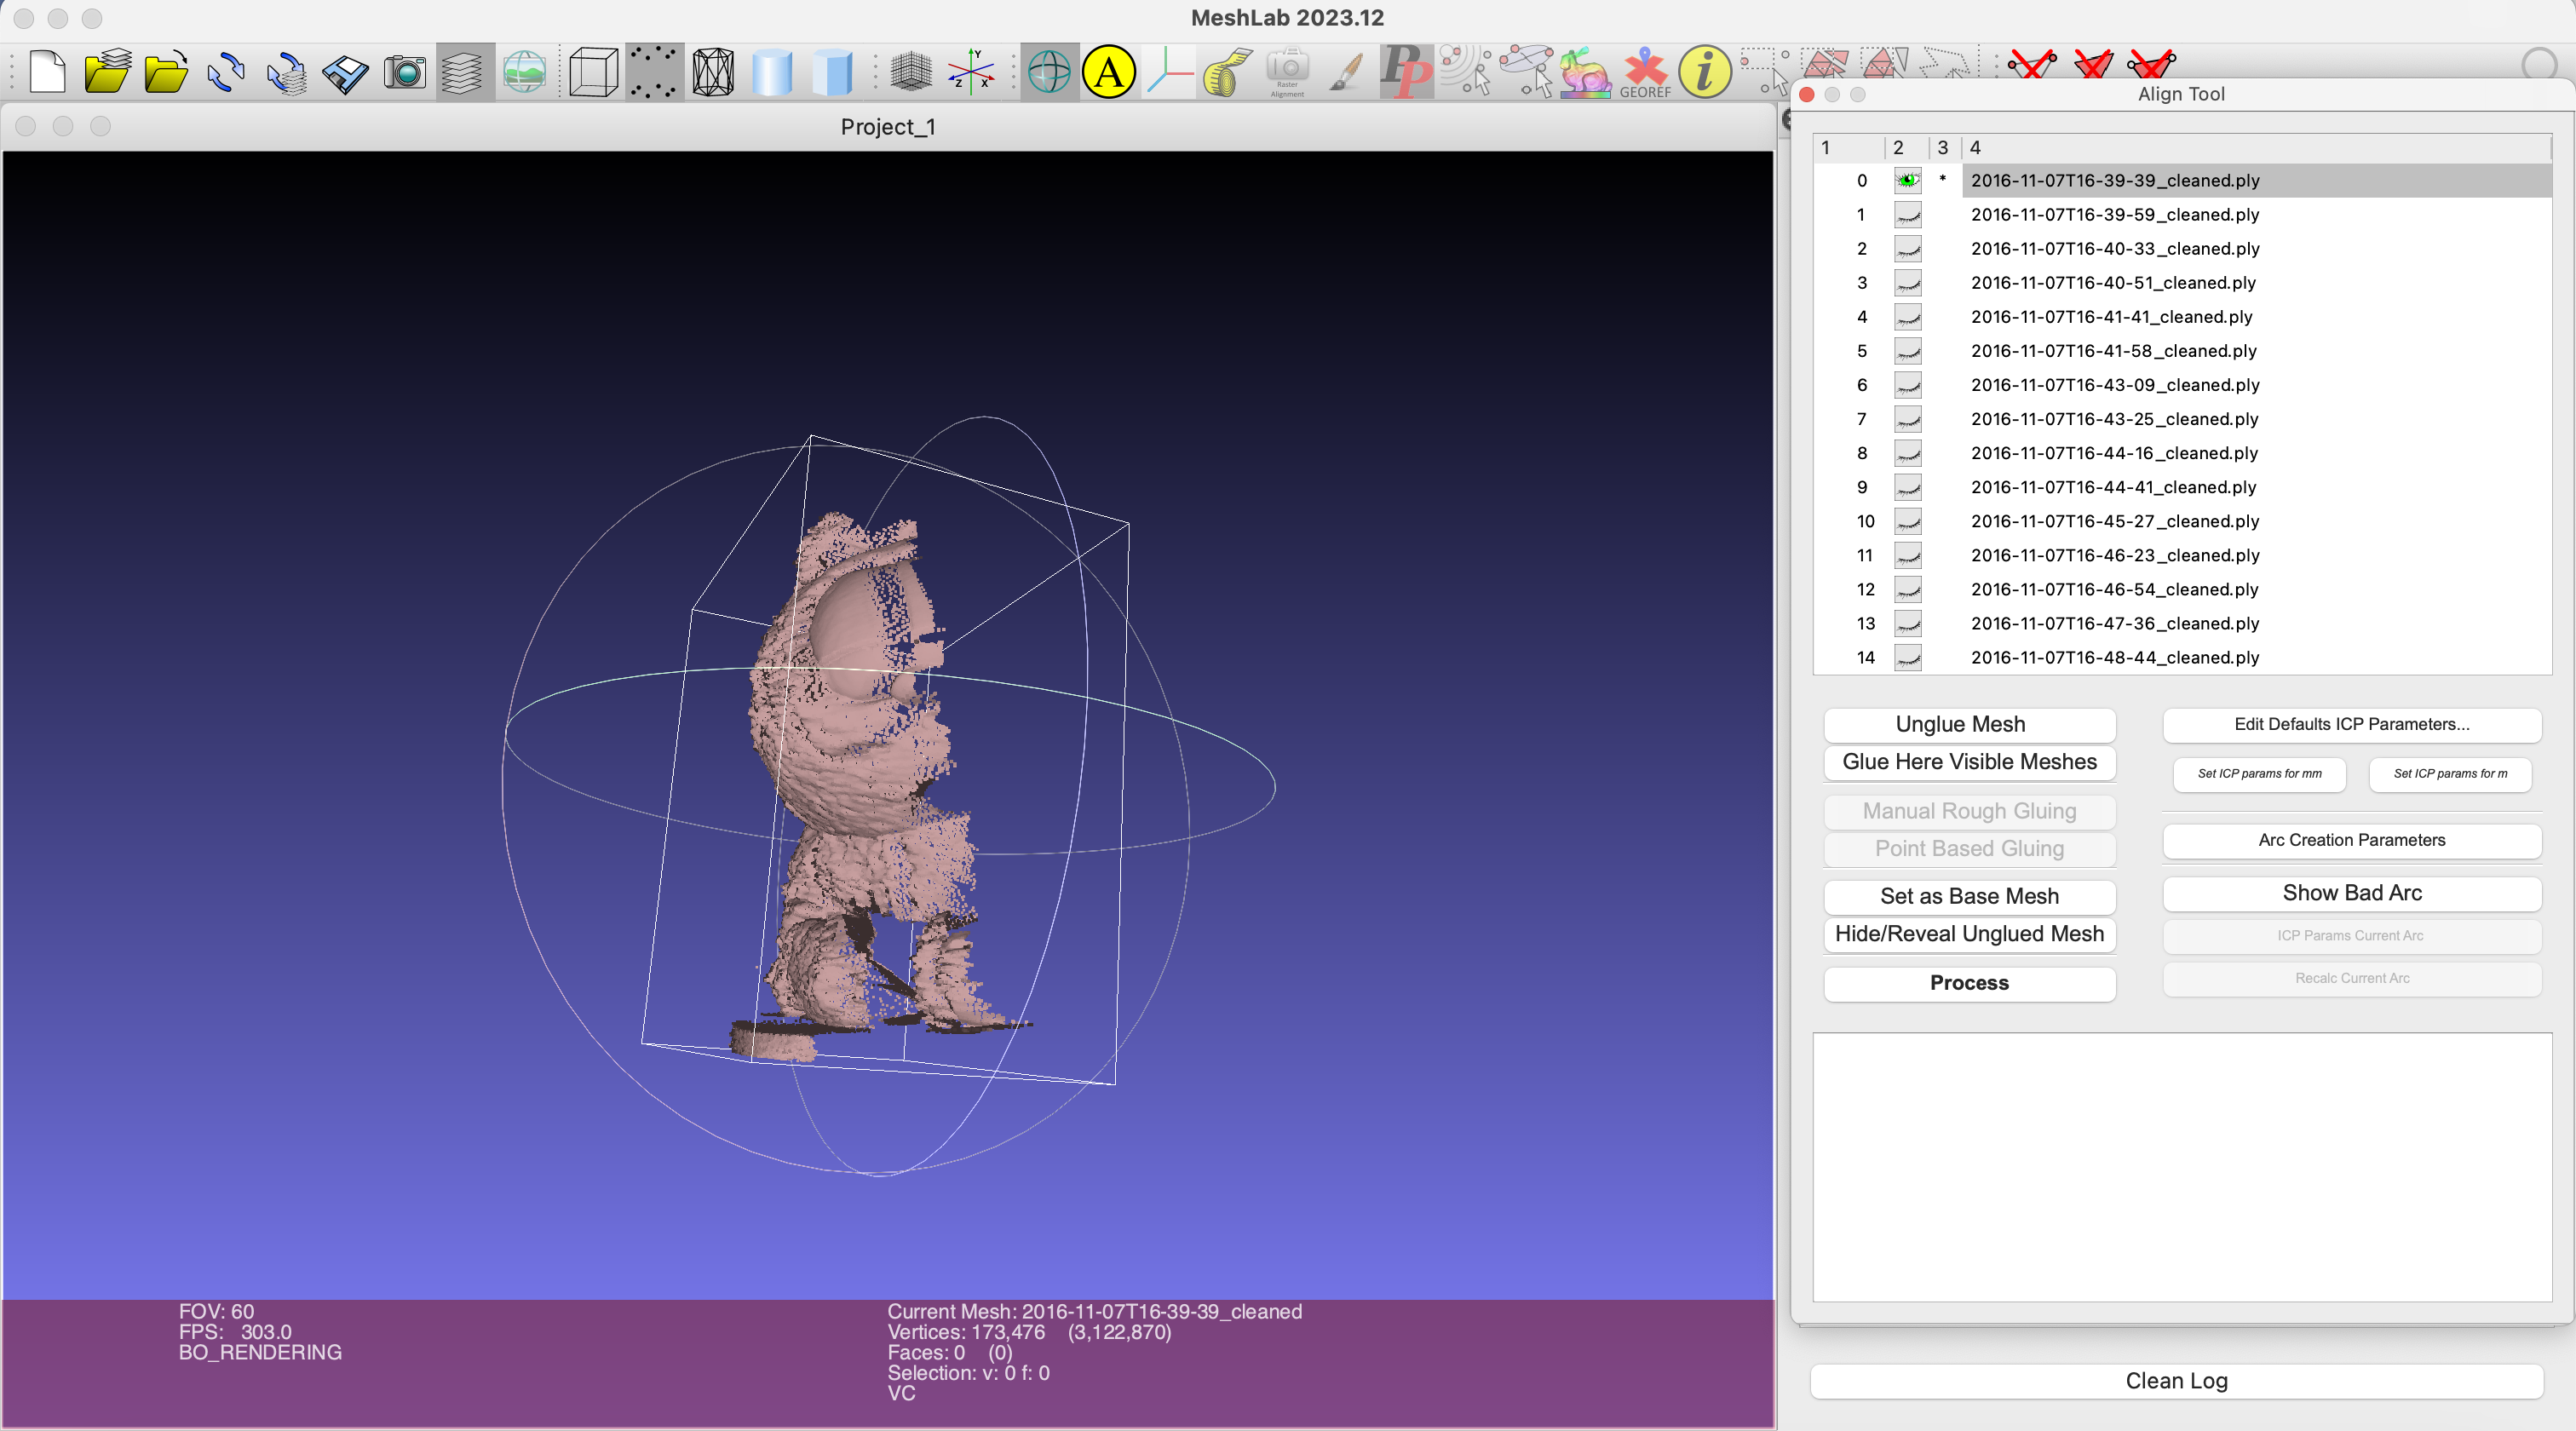
\includegraphics[width=1\textwidth]{screenshots/4.png}
			\caption{Prikazan je prvi layer}
			\label{fig:yourlabel}
		\end{figure}
		Zatim kliknemo na layer ispod i odaberemo Point Based Gluing. Moramo sad spojiti parove odgovarajućih točaka i kliknuti OK.		\begin{figure}[H]
			\centering
			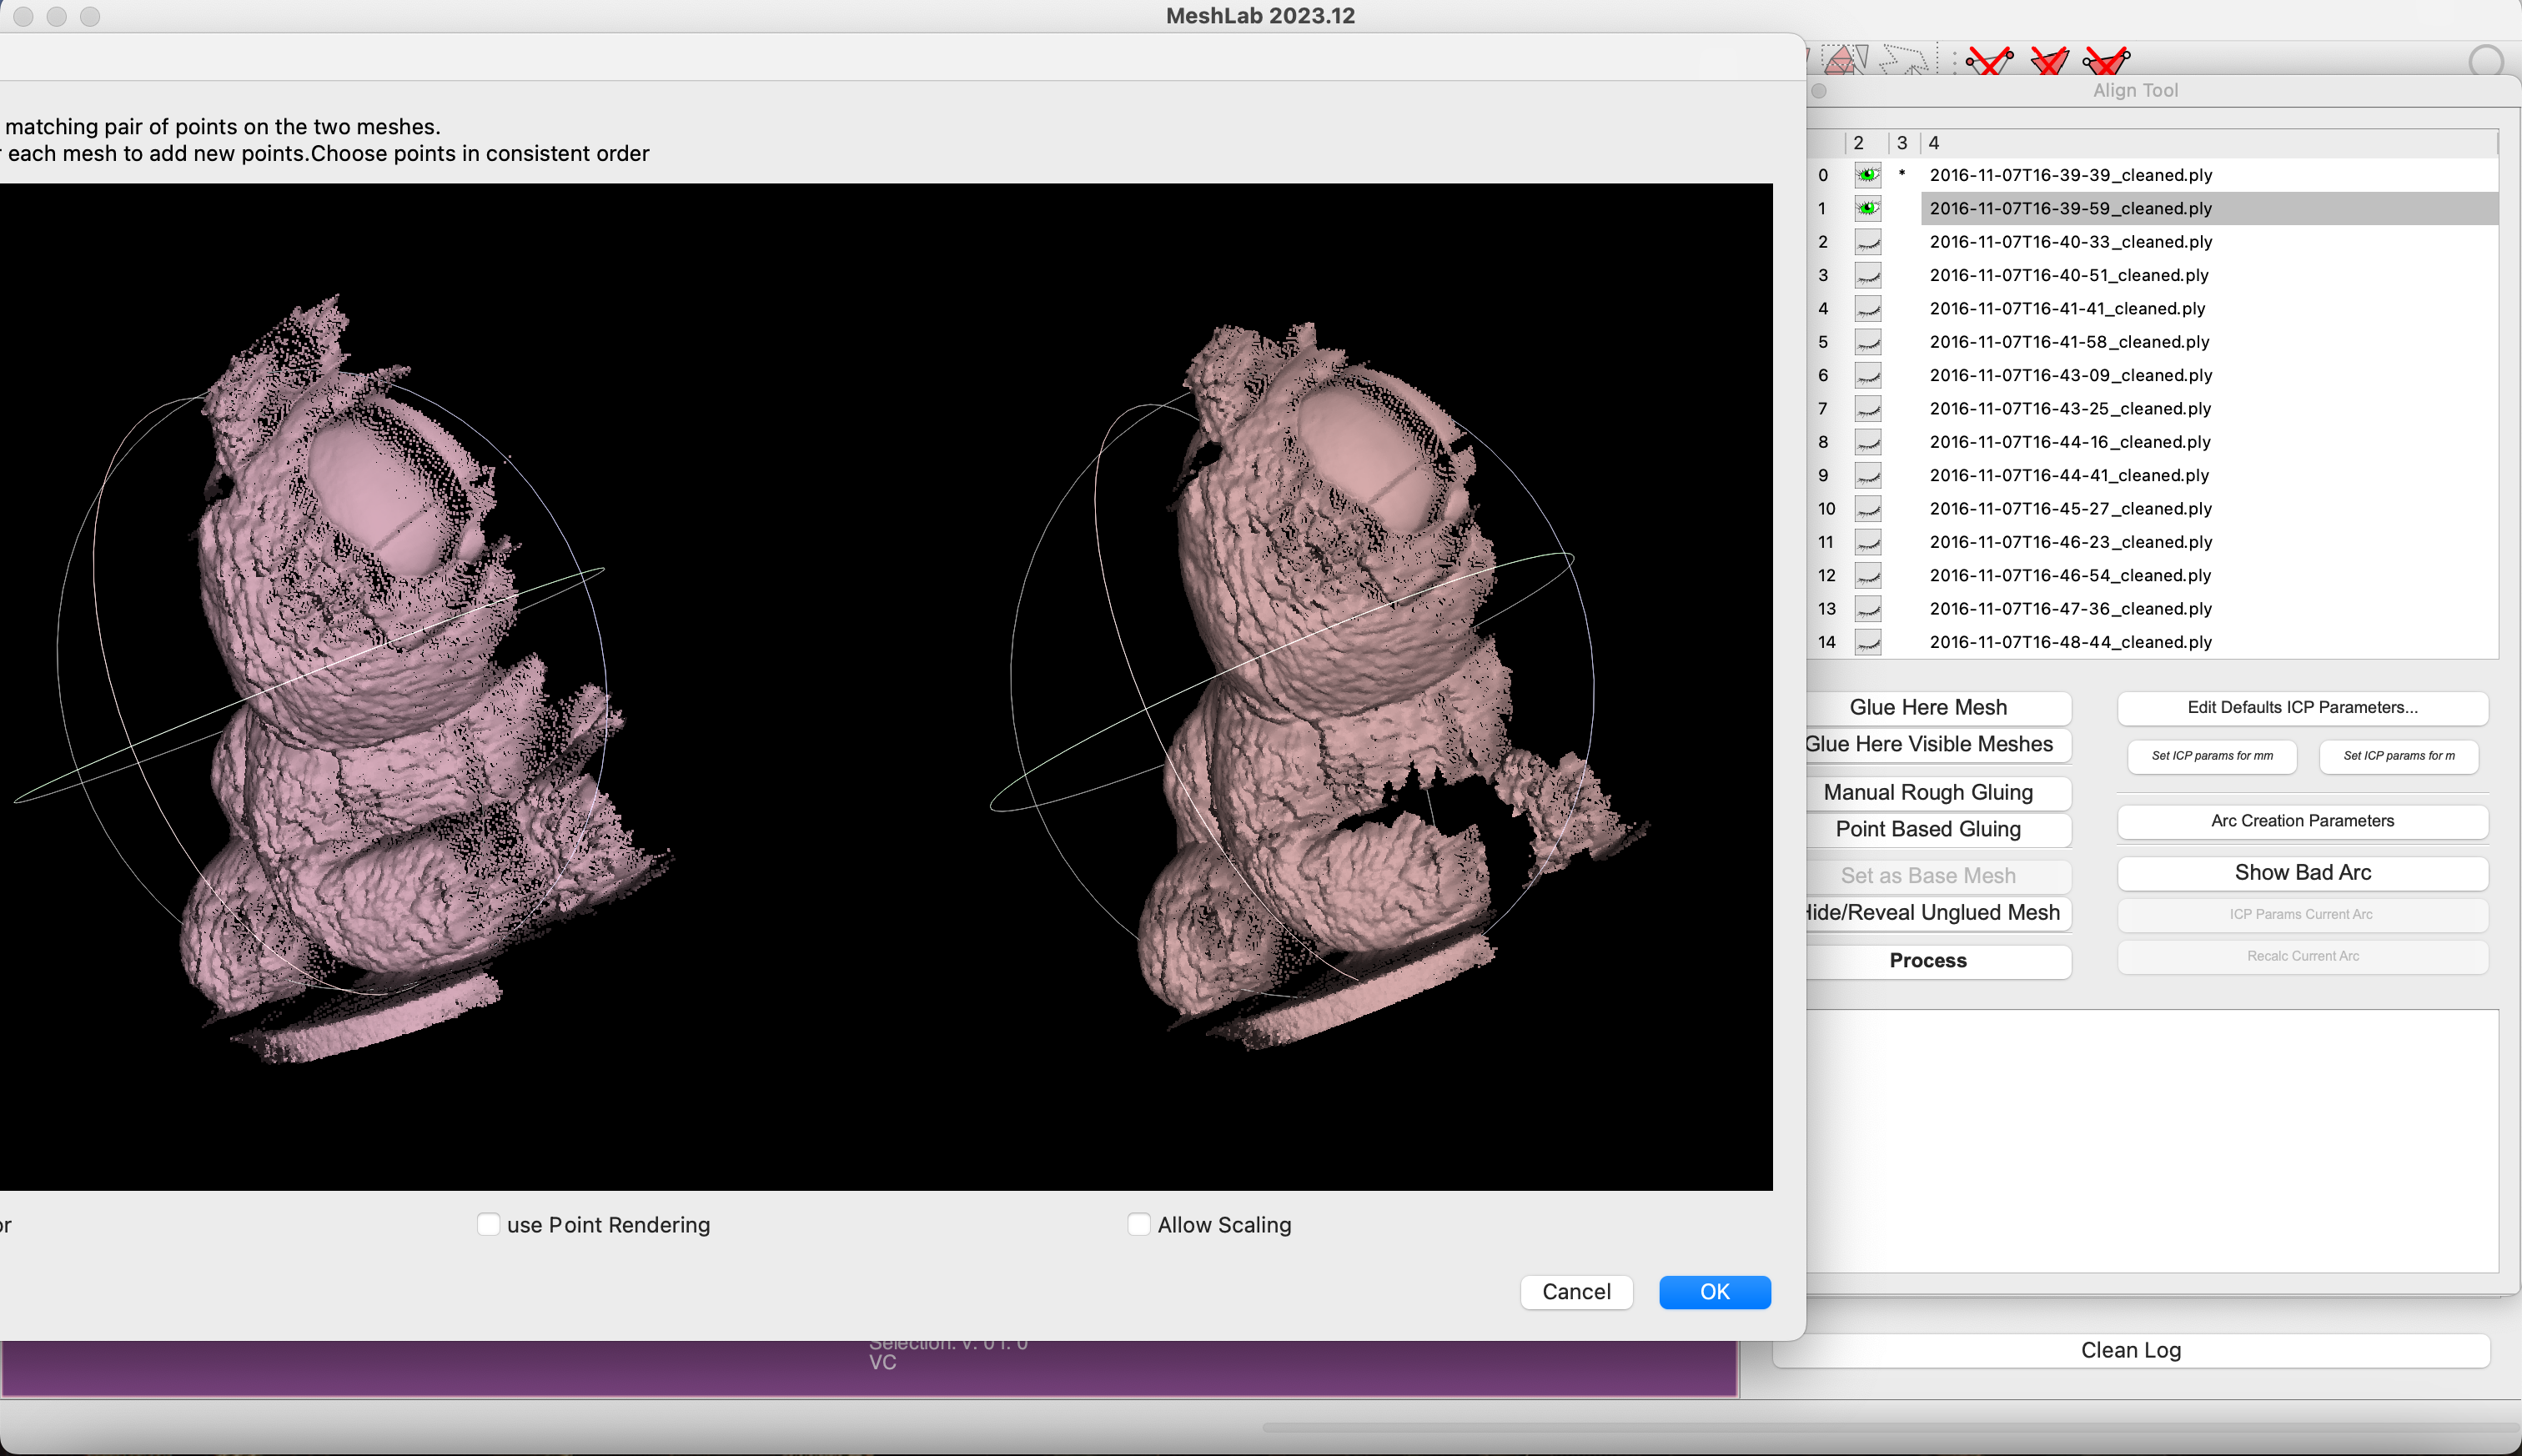
\includegraphics[width=0.9\textwidth]{screenshots/5.png}
			\caption{Spajanje točaka}
			\label{fig:yourlabel}
		\end{figure}
		
		Isti postupak ponovimo za sljedeće meshove.
		\begin{figure}[H]
			\centering
			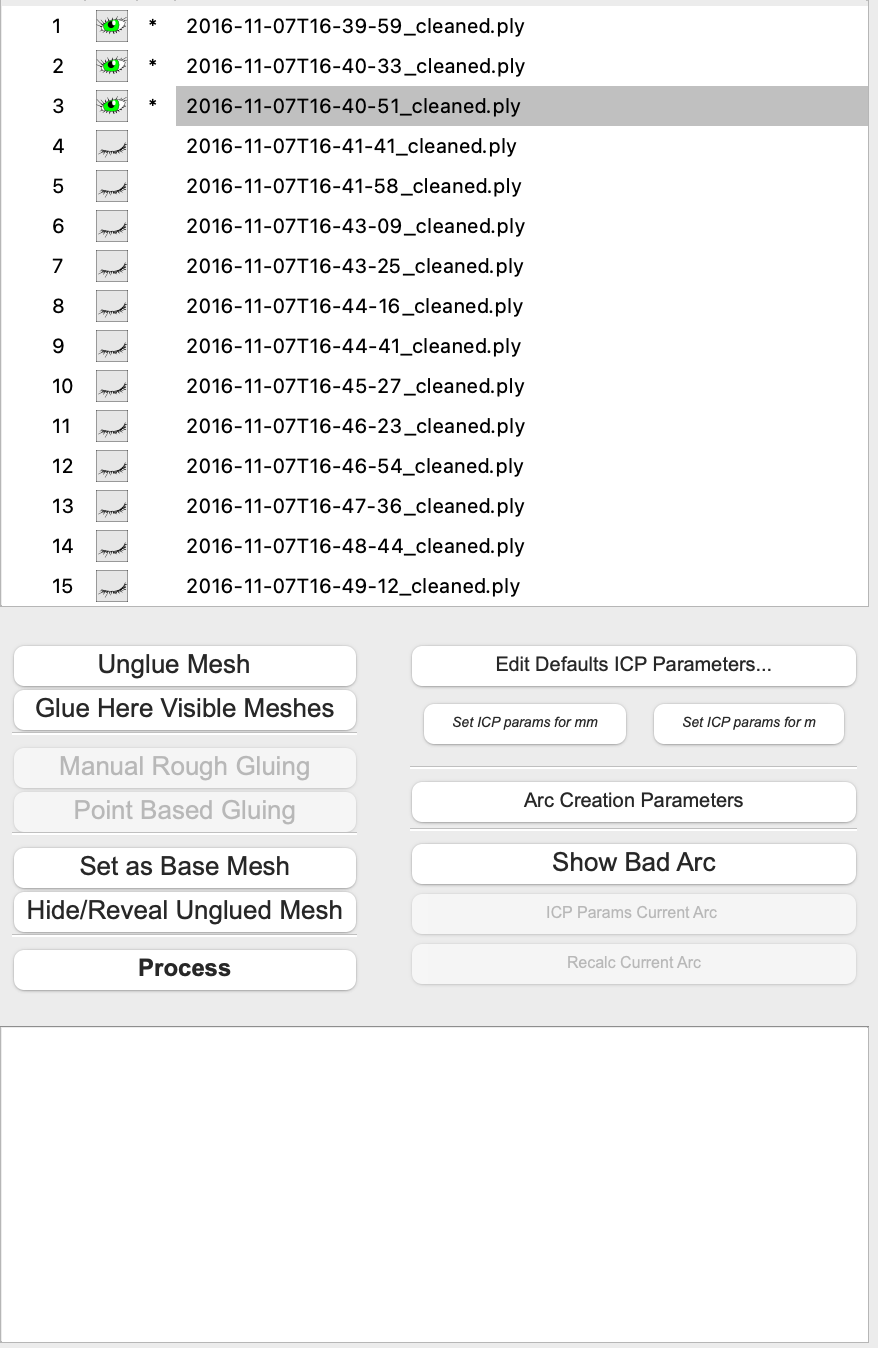
\includegraphics[width=0.4\textwidth]{screenshots/6.png}
			\caption{Ostali meshevi}
			\label{fig:yourlabel}
		\end{figure}
		
		Nakon sljedećih postupaka, kliknemo Process kako bi izvršili globalno poravnanje svih mesheva dosad.
		
		\begin{figure}[H]
			\centering
			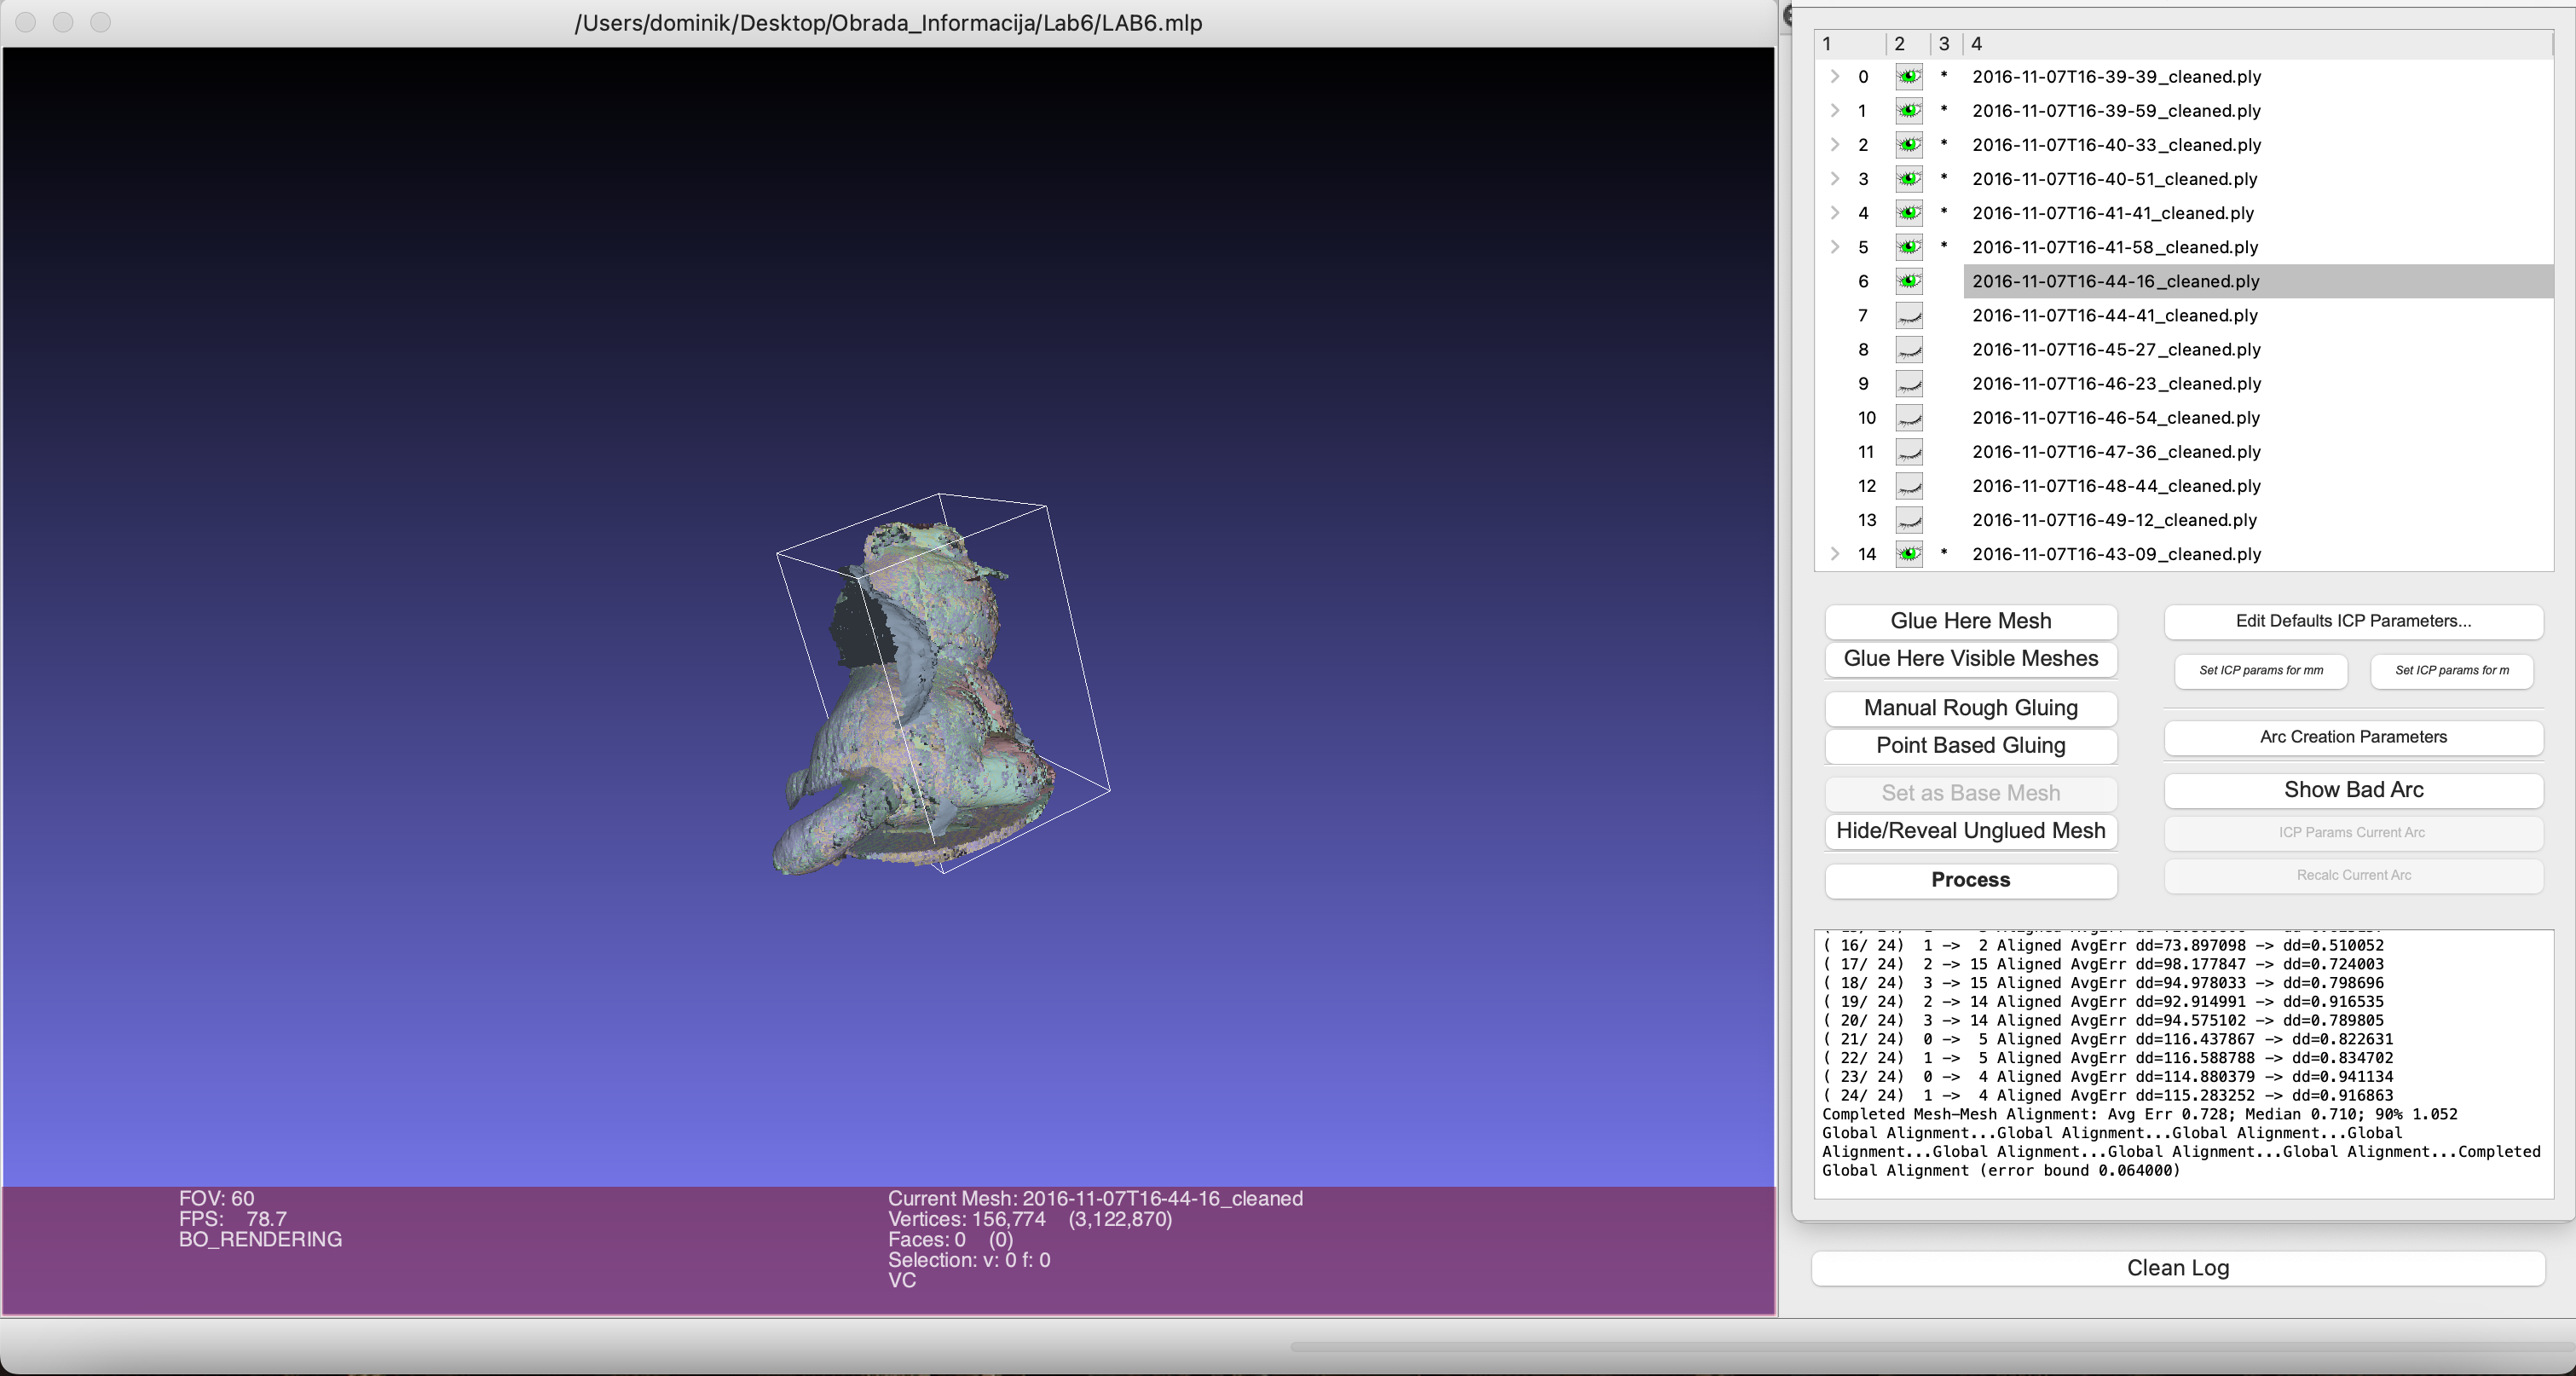
\includegraphics[width=1\textwidth]{screenshots/8.png}
			\caption{Global Alignment}
			\label{fig:yourlabel}
		\end{figure}
		
		Nastavljamo postupak spajanja točaka. Objekt je sve više potpun.
		\begin{figure}[H]
			\centering
			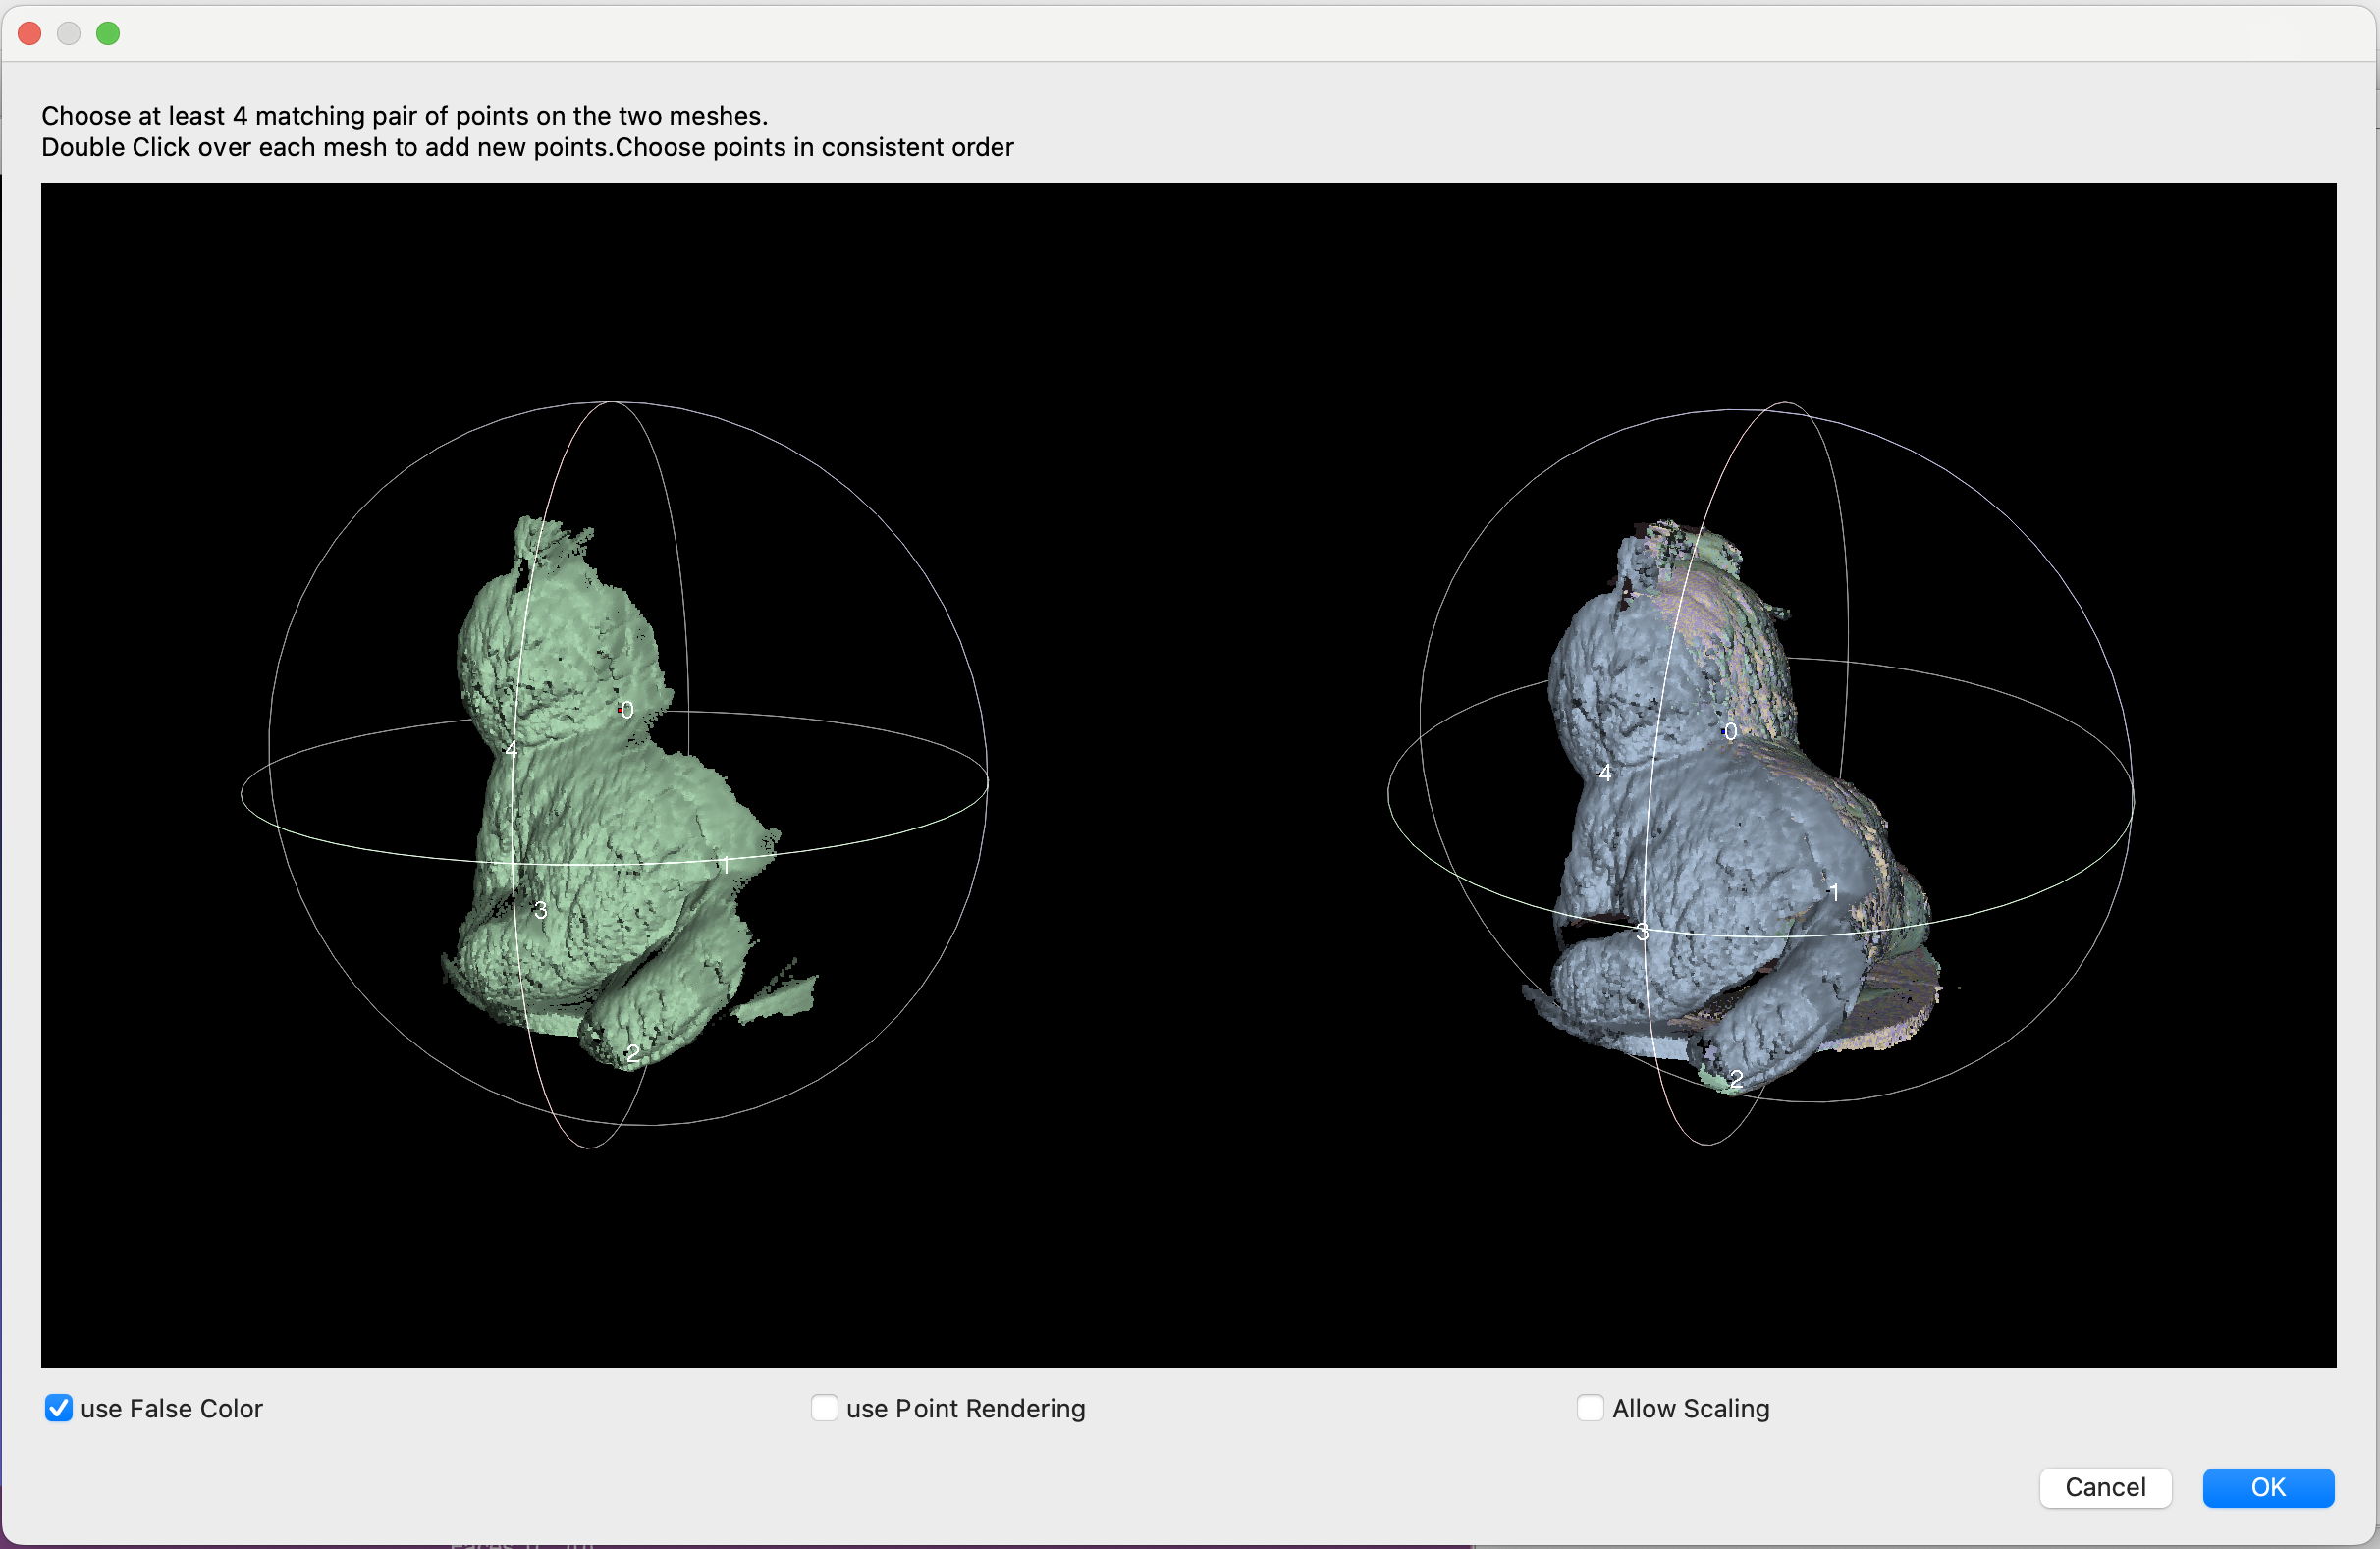
\includegraphics[width=1\textwidth]{screenshots/9.png}
			\caption{Spajanje novog mesha uz ostale}
			\label{fig:yourlabel}
		\end{figure}
		
		Sada ćemo Ungluati dosta prvih mesheva, i nastavit ćemo rad uz zadnja 2 poravnana mesha kako bi mogli koristiti algoritam ICP u poravnanju, jer za previše mesheva se aplikacija ugasi sama od sebe.
		\begin{figure}[H]
			\centering
			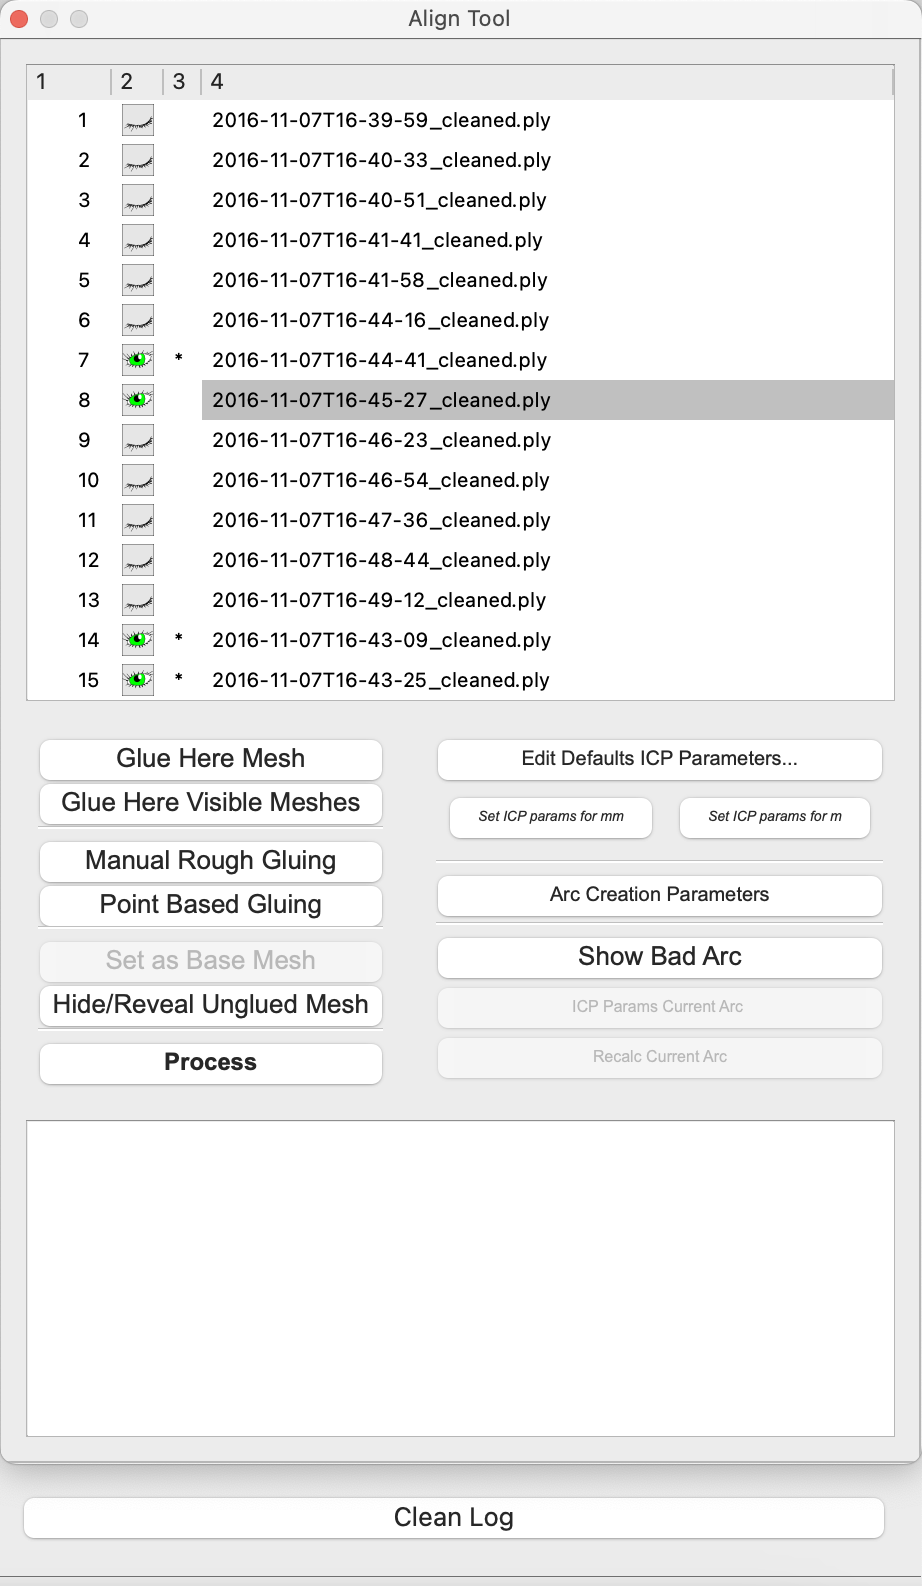
\includegraphics[width=0.3\textwidth]{screenshots/10.png}
			\caption{Nastavak postupka}
			\label{fig:yourlabel}
		\end{figure}
		
		Postupak ponavljamo dok ne upotpunimo objekt.
		
		\begin{figure}[H]
			\centering
			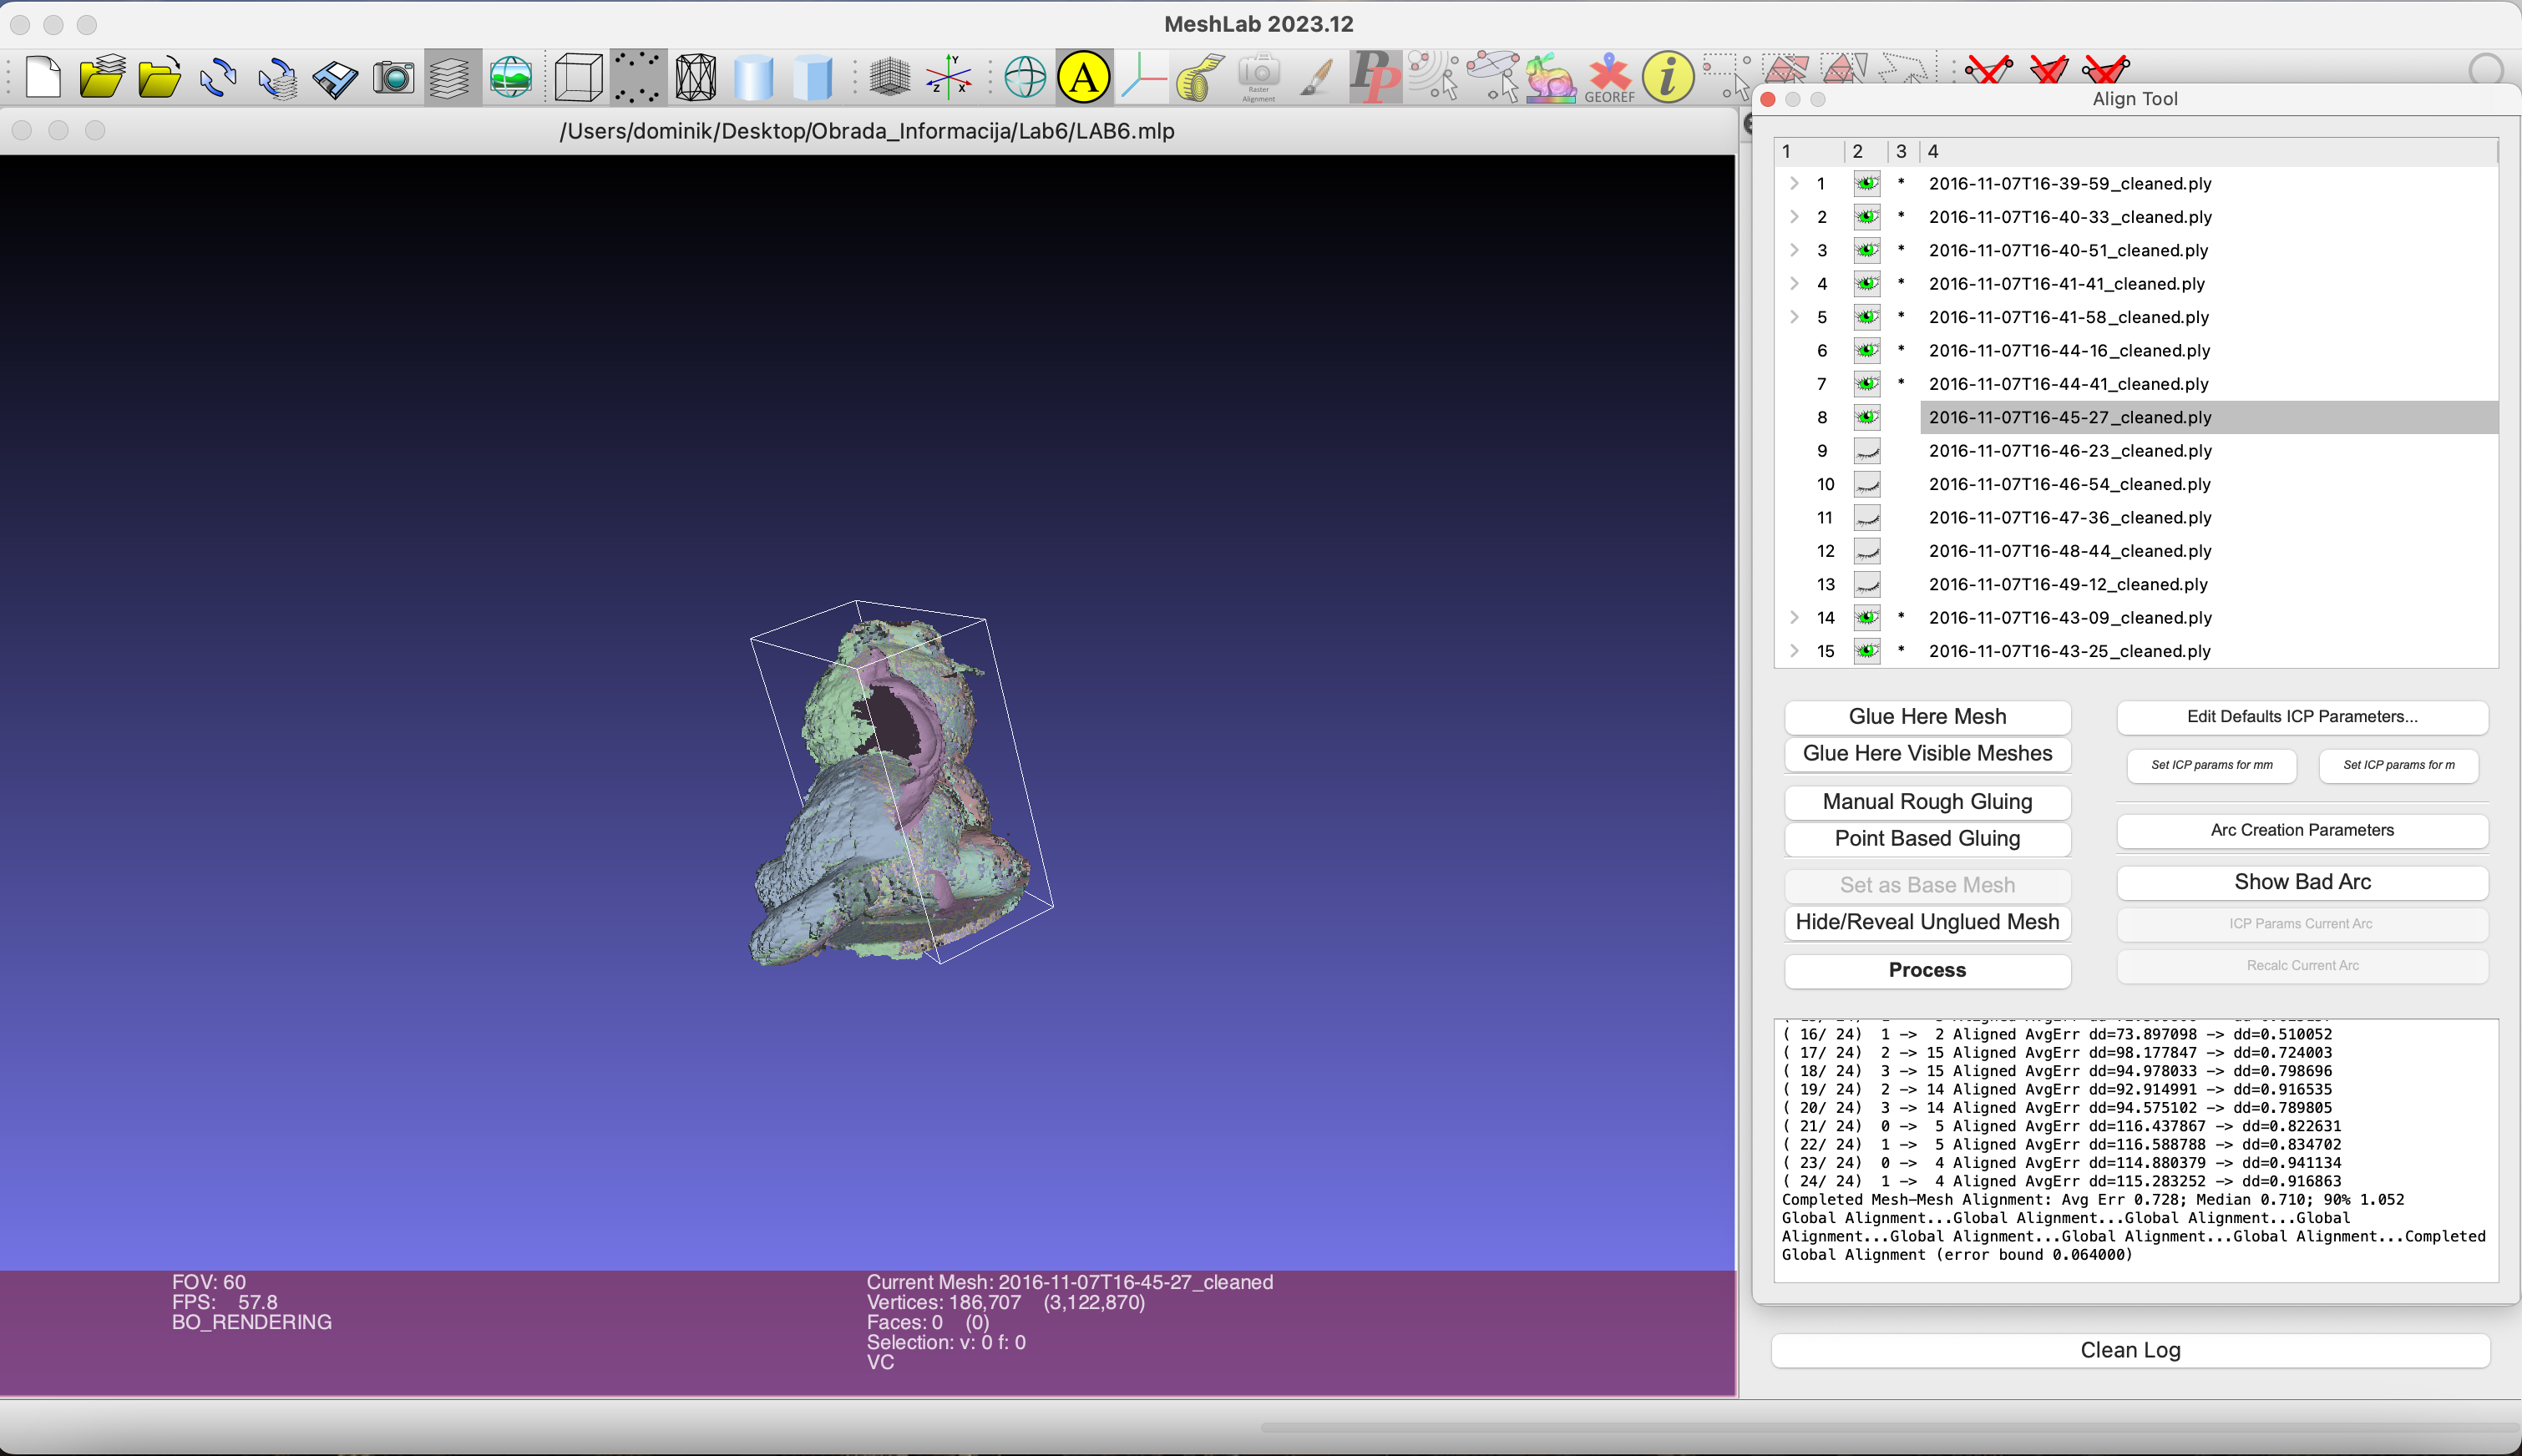
\includegraphics[width=1\textwidth]{screenshots/11.png}
			\caption{Postepeno upotpunjavanje objekta}
			\label{fig:yourlabel}
		\end{figure}
		
		\begin{figure}[H]
			\centering
			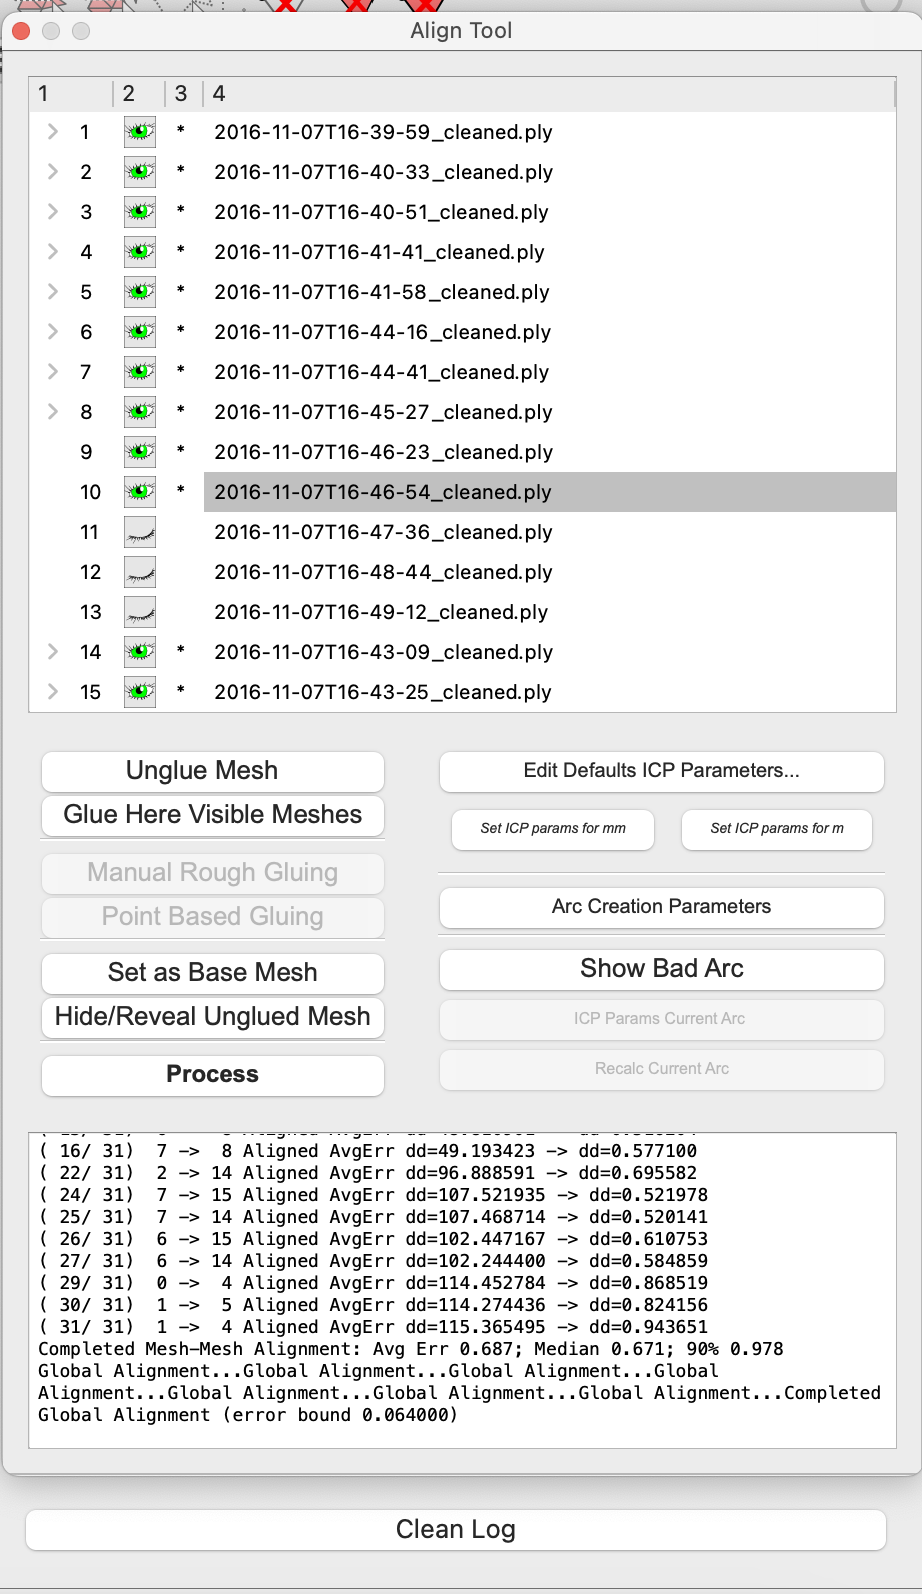
\includegraphics[width=0.3\textwidth]{screenshots/12.png}
			\caption{Vidimo sve više glueanih mesheva}
			\label{fig:yourlabel}
		\end{figure}
		
		Kada zavrsimo poravnavanje svih mesheva, dobijemo ovakav objekt, slika je na sljedećoj strani.
		
		\begin{figure}[H]
			\centering
			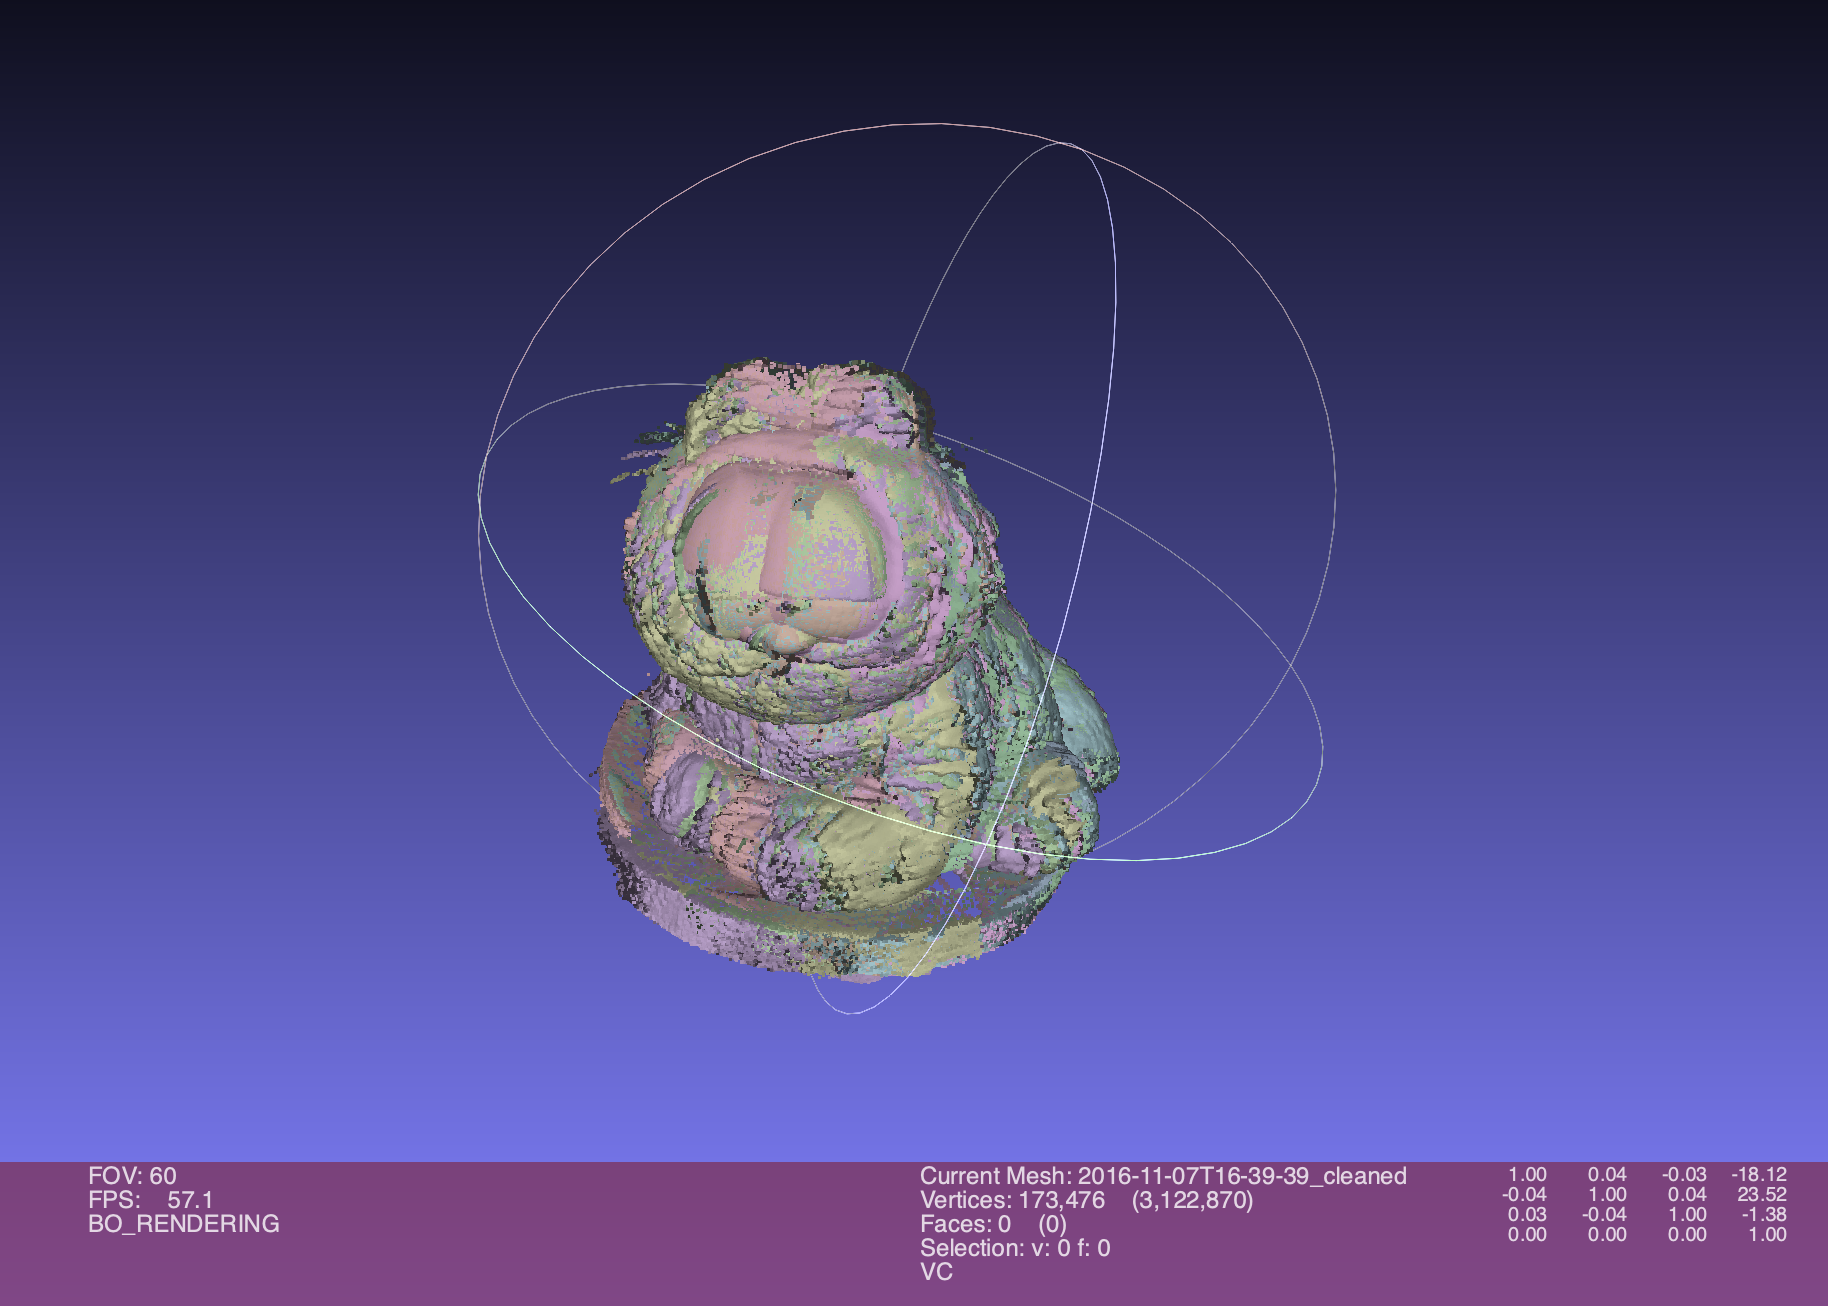
\includegraphics[width=0.65\textwidth]{screenshots/16.png}
			\caption{Garfield}
			\label{fig:yourlabel}
		\end{figure}
		
		Sada je potrebno povezaati sve layere/mesheve u jedan mesh.
		Odaberemo Filters - Mesh Layer - Flatten Visible Layers.
		
		\begin{figure}[H]
			\centering
			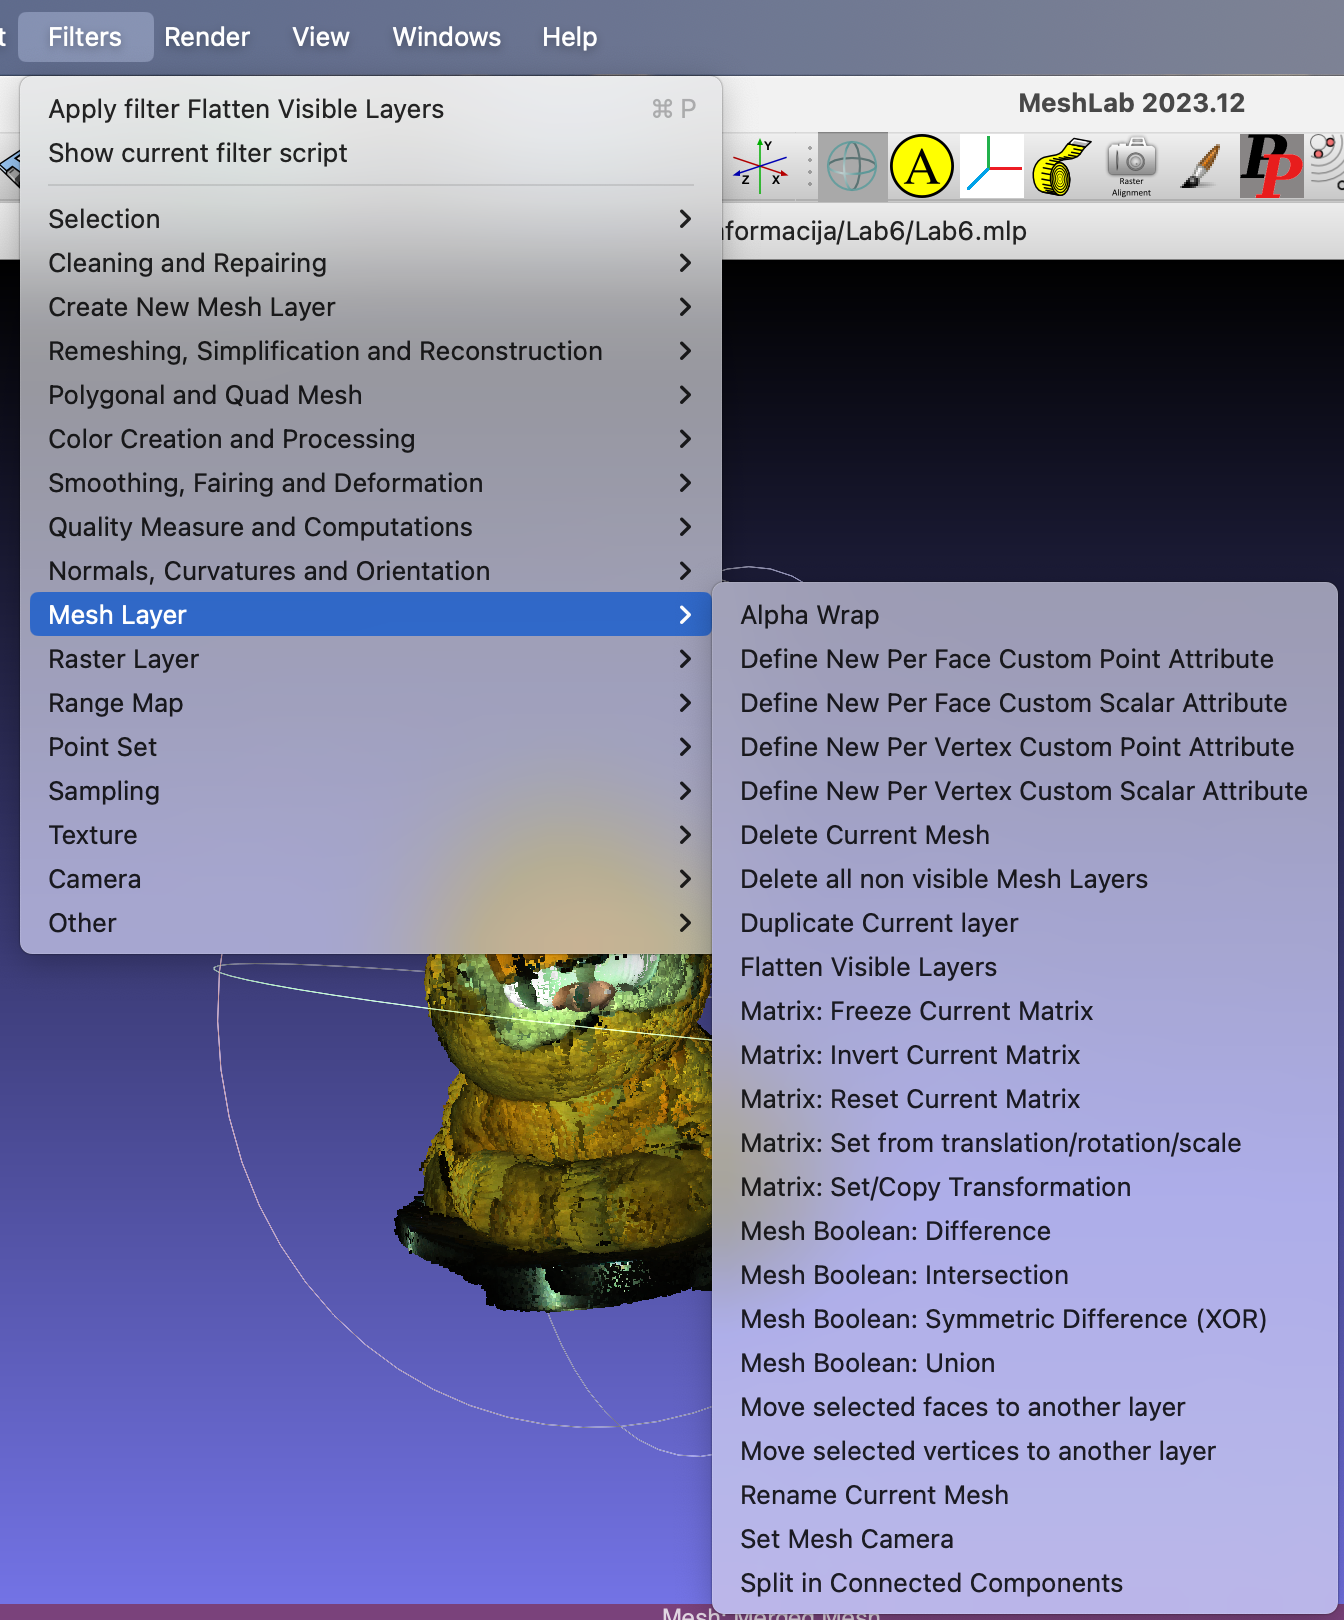
\includegraphics[width=0.7\textwidth]{screenshots/17.png}
			\caption{Flattened Meshes into one Mesh Object}
			\label{fig:yourlabel}
		\end{figure}

		\begin{figure}[H]
			\centering
			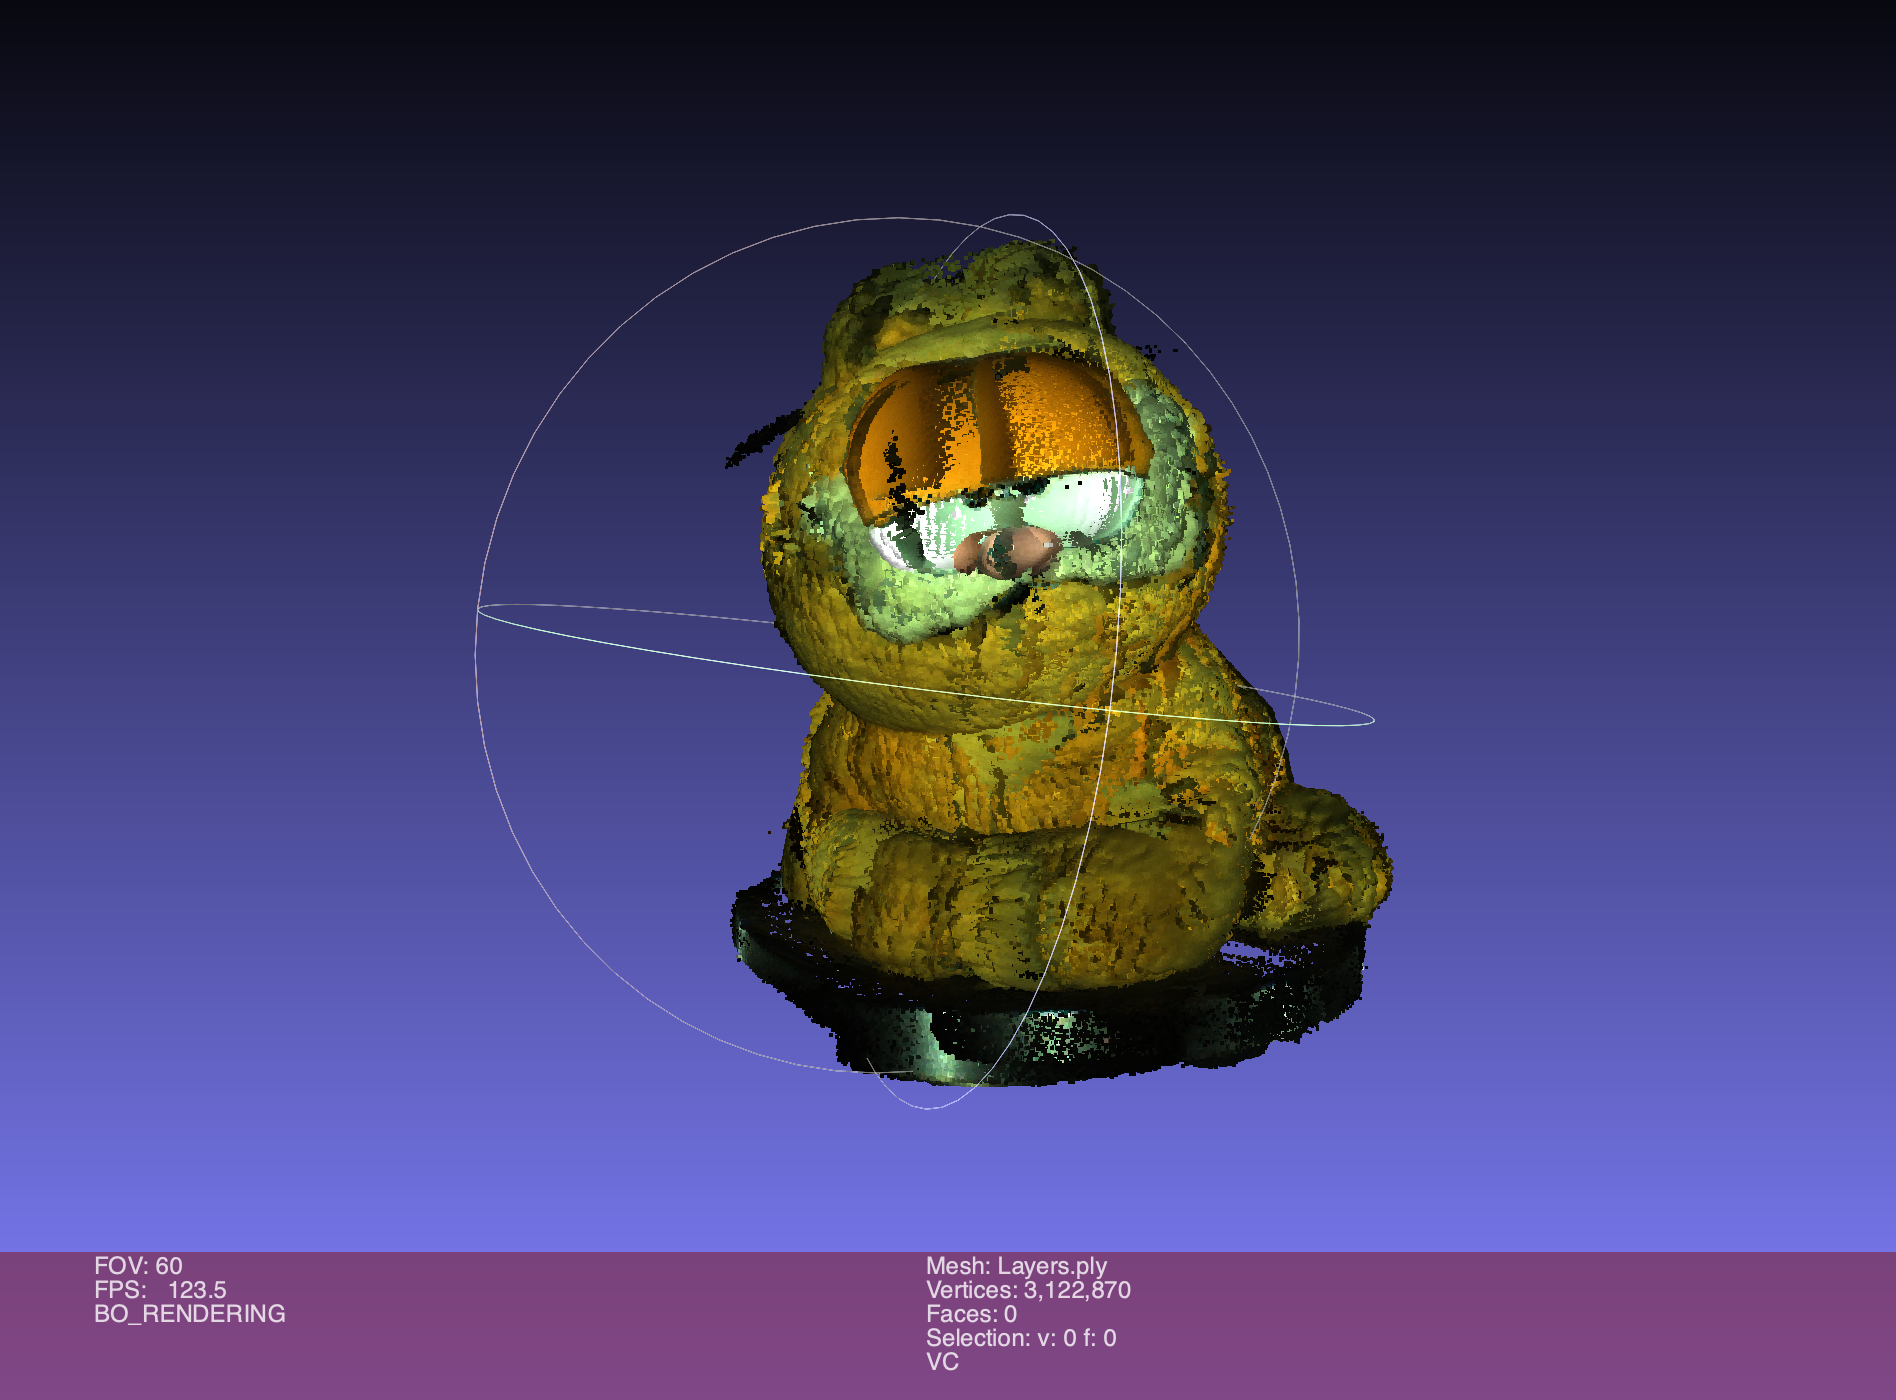
\includegraphics[width=0.7\textwidth]{screenshots/18.png}
			\caption{Ovo je konačni rezultat poravnanja i flattenanja}
			\label{fig:yourlabel}
		\end{figure}
				Sada exportamo taj mesh kao .ply datoteku
		\begin{figure}[H]
			\centering
			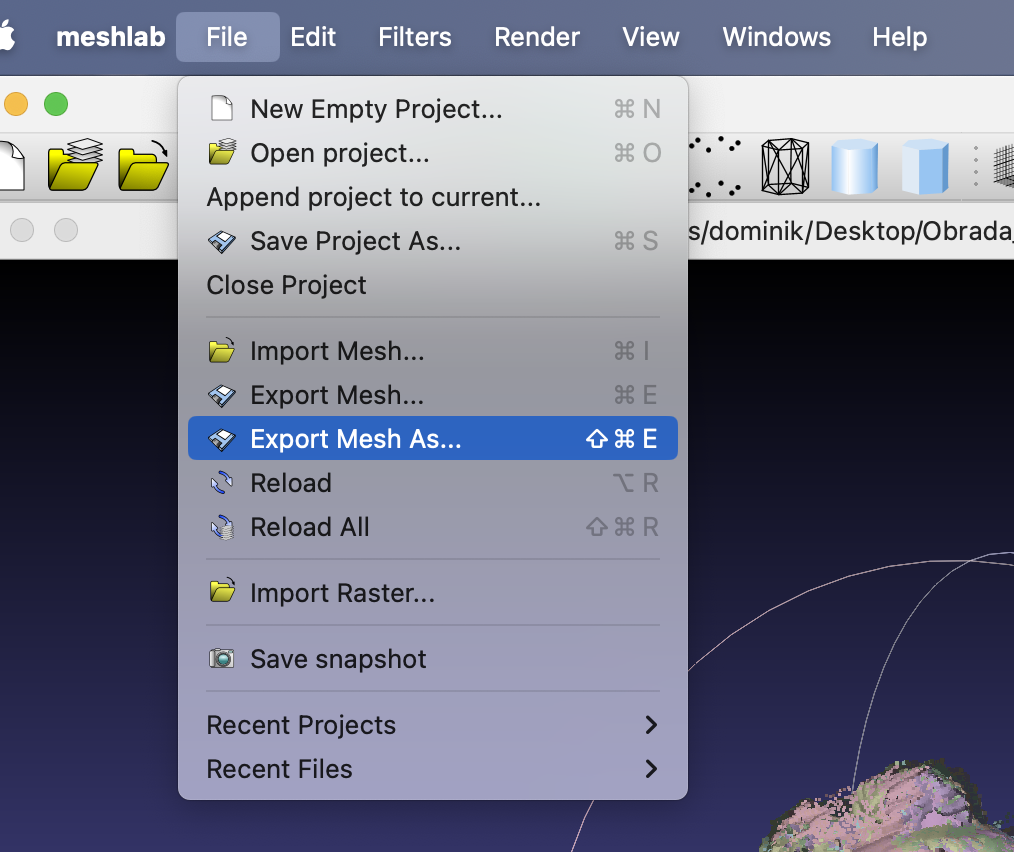
\includegraphics[width=0.65\textwidth]{screenshots/19.png}
			\caption{Export Mesh}
			\label{fig:yourlabel}
		\end{figure}
		
	\eject
	
	\pagebreak
	\section{Zaključak}
	S obzirom na to da exportani mesh ima preveliku veličinu u MB, moramo obaviti Surface Reconstruction za smanjenje veličine na do 15MB.

		\begin{figure}[H]
			\centering
			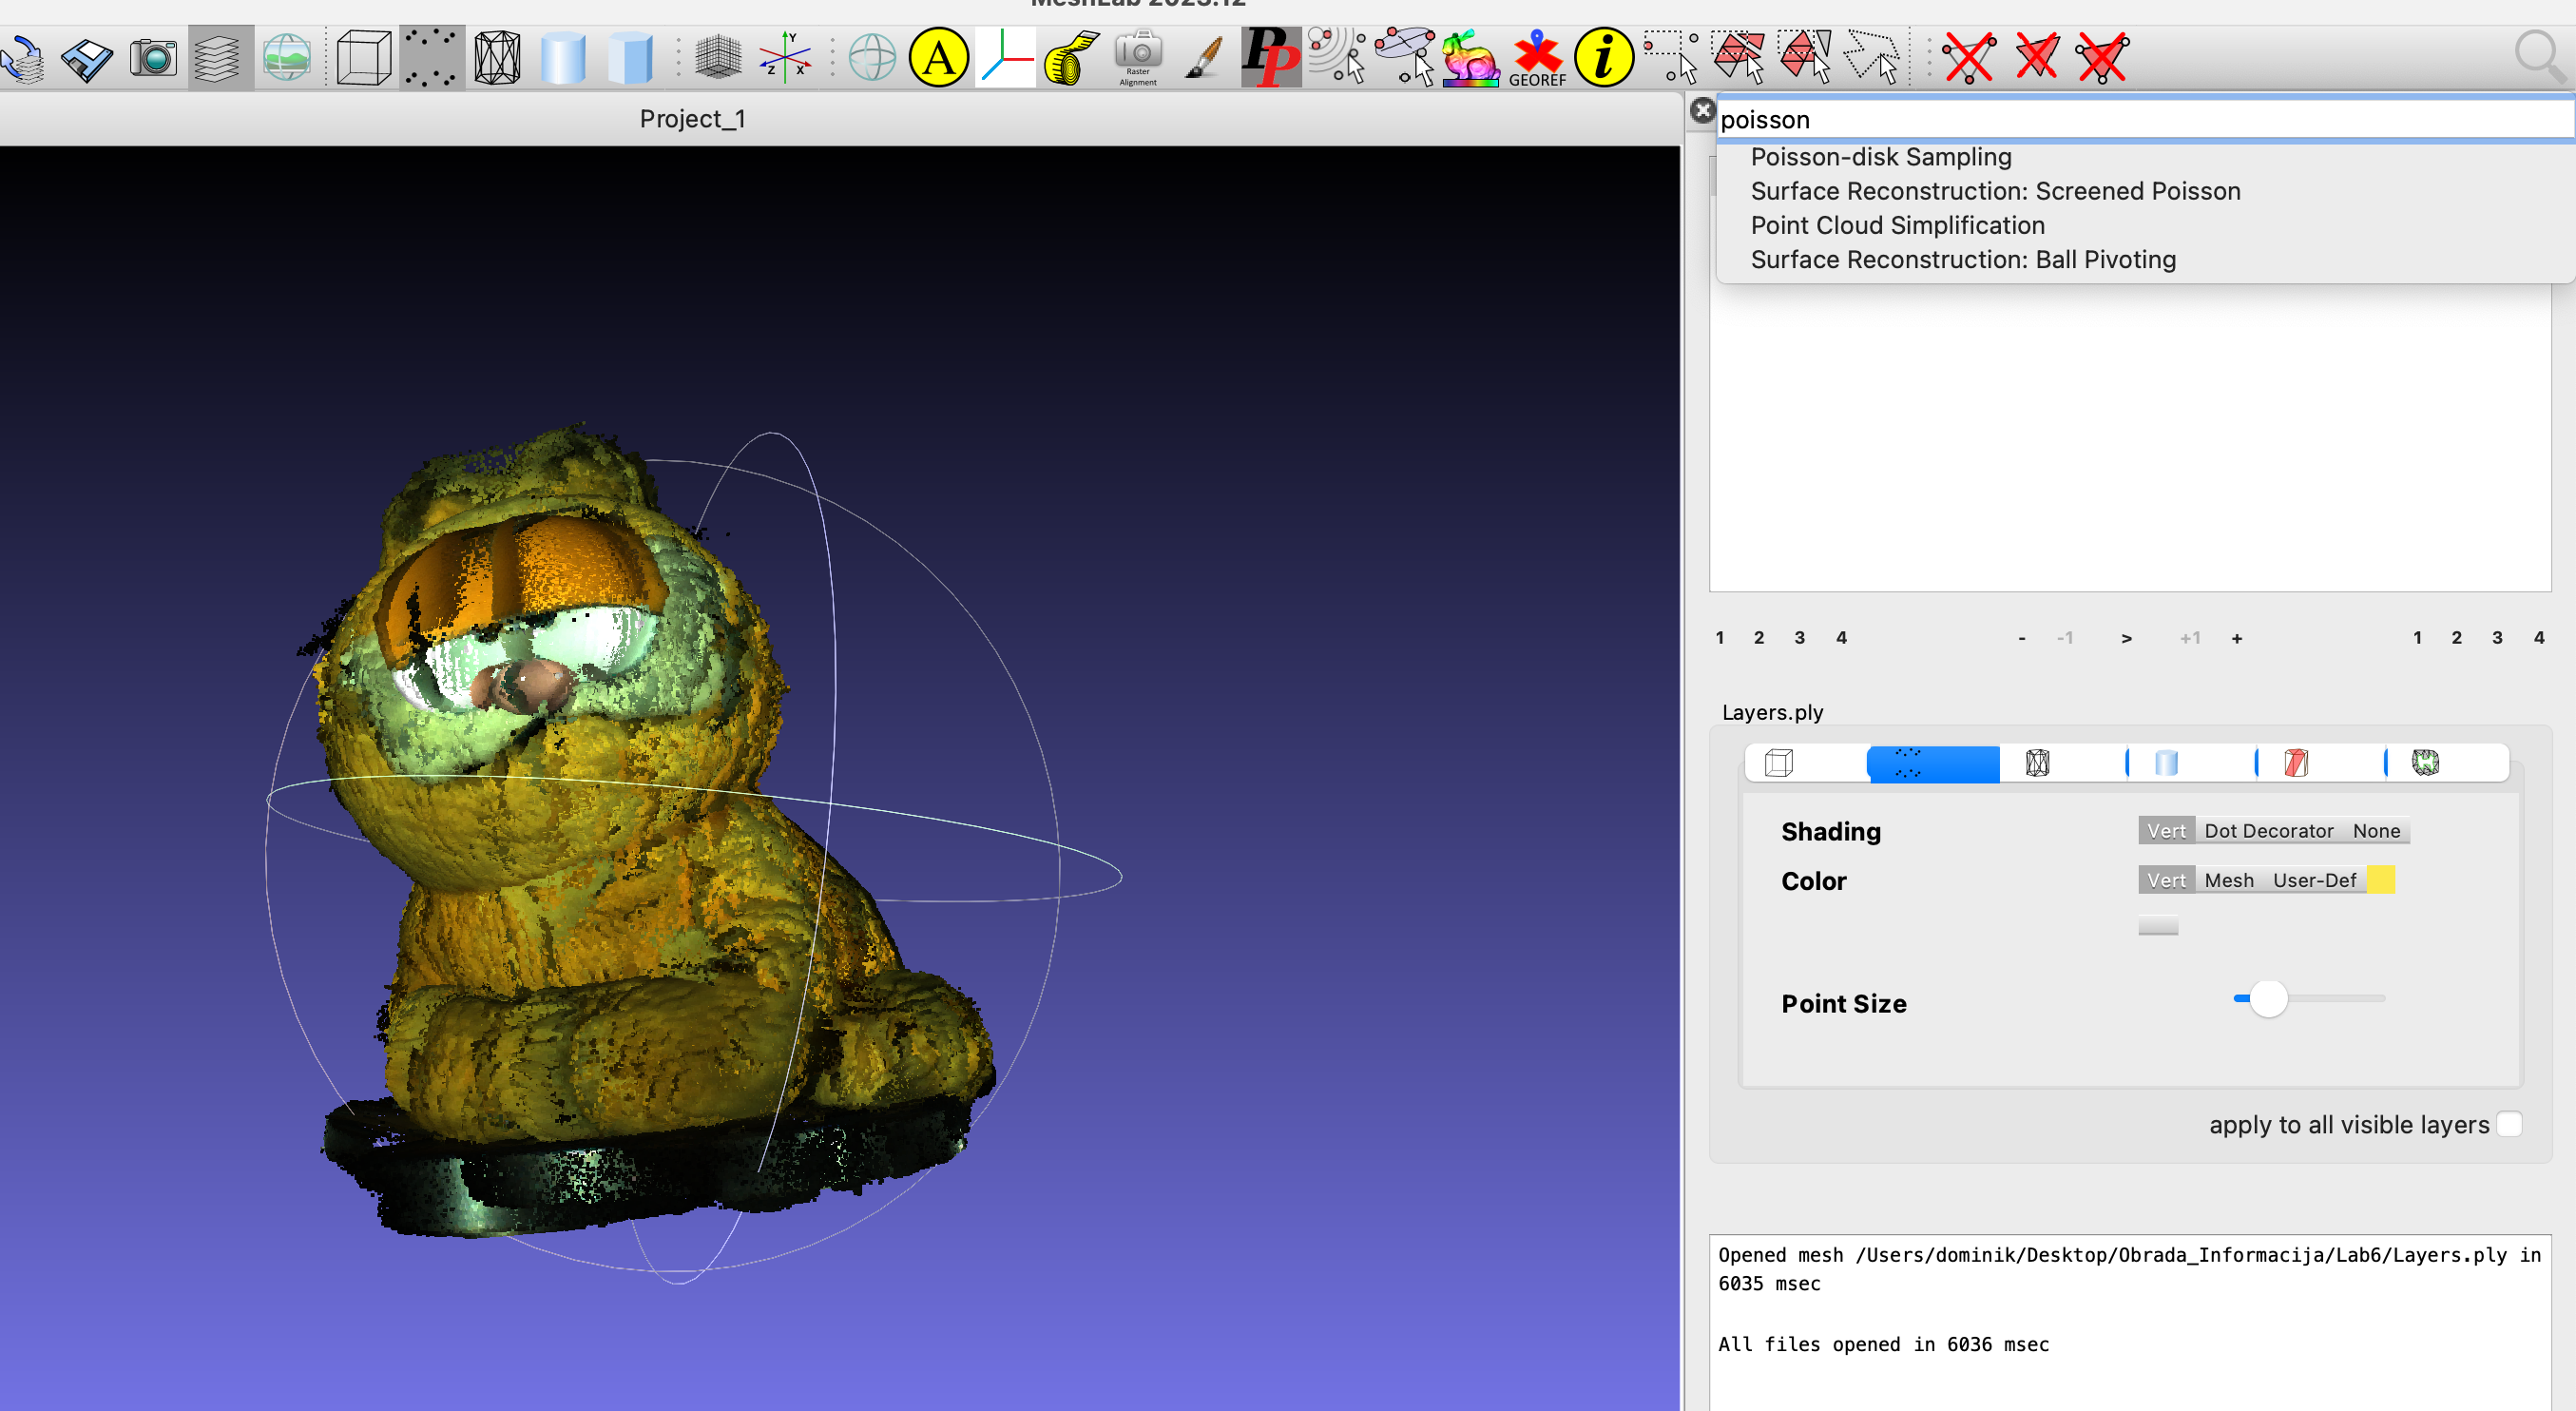
\includegraphics[width=0.7\textwidth]{screenshots/20.png}
			\caption{Prikazan je mesh koji treba obraditi}
			\label{fig:yourlabel2}
		\end{figure}
		
		Ostavimo ove parametre koji su defaultni i kliknemo Apply te čekamo da se završi proces.
		\begin{figure}[H]
			\centering
			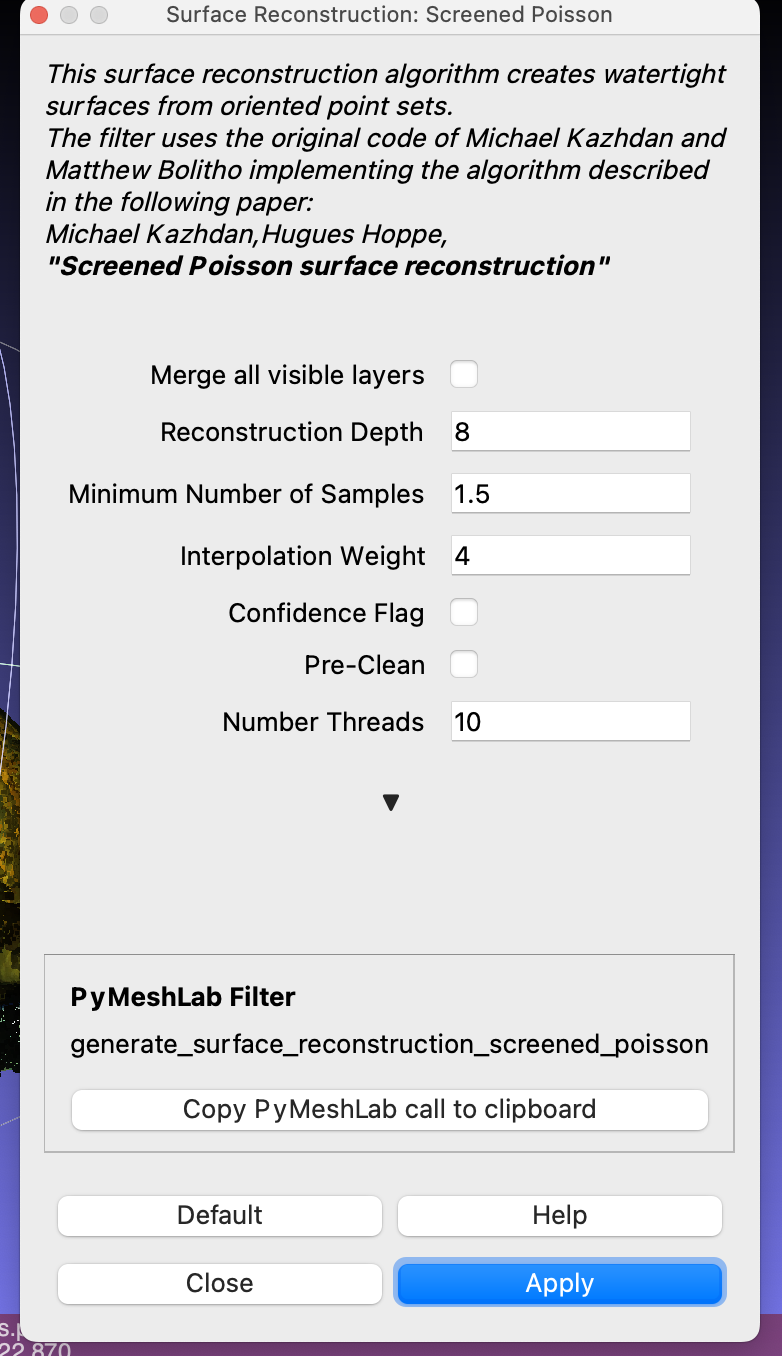
\includegraphics[width=0.4\textwidth]{screenshots/21.png}
			\caption{Surface Reconstruction parametri}
			\label{fig:yourlabel2}
		\end{figure}
		
		
		\begin{figure}[H]
			\centering
			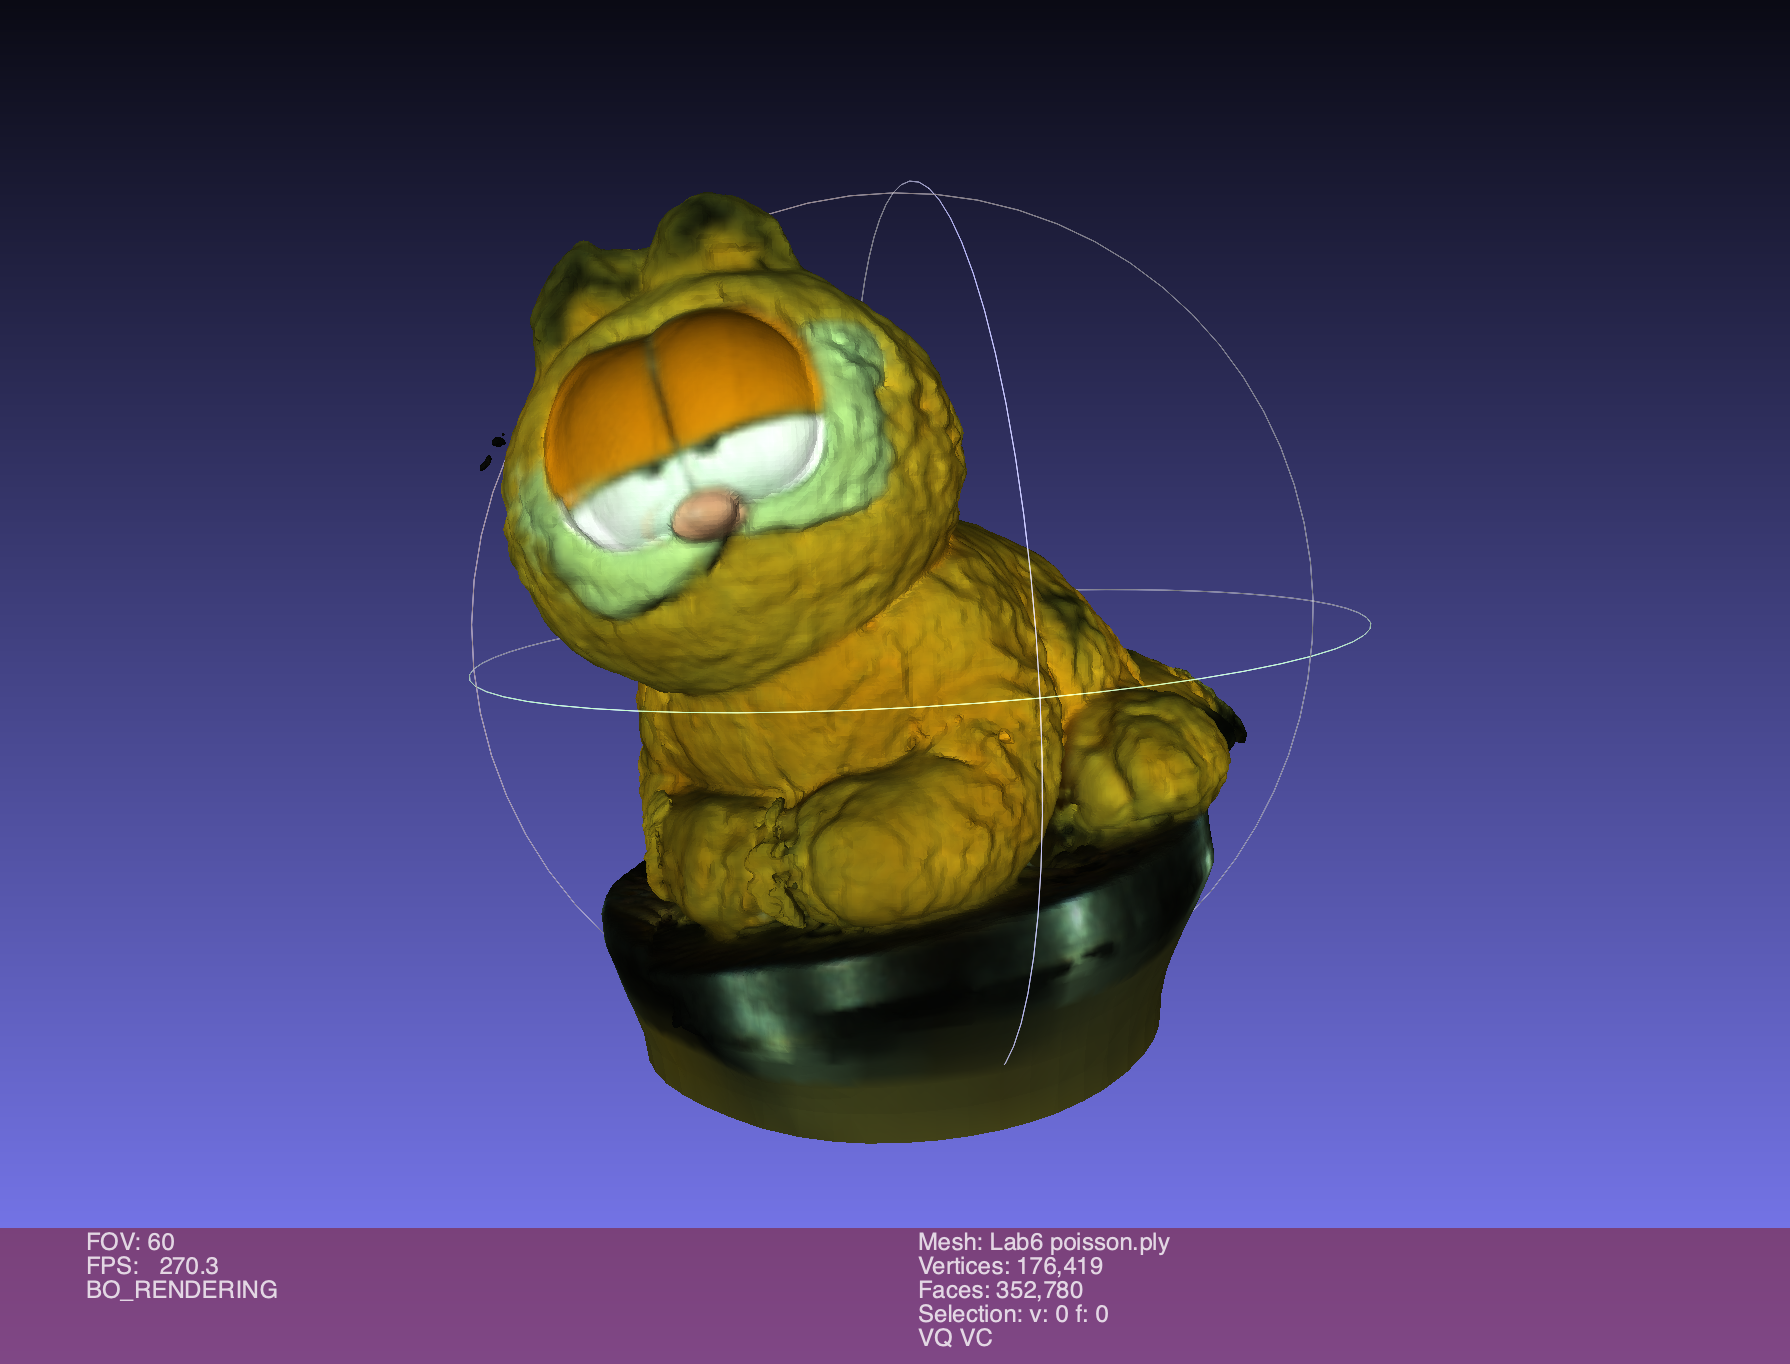
\includegraphics[width=0.8\textwidth]{screenshots/22.png}
			\caption{Konačan rezultat 1}
			\label{fig:yourlabel2}
		\end{figure}
		
		
		\begin{figure}[H]
			\centering
			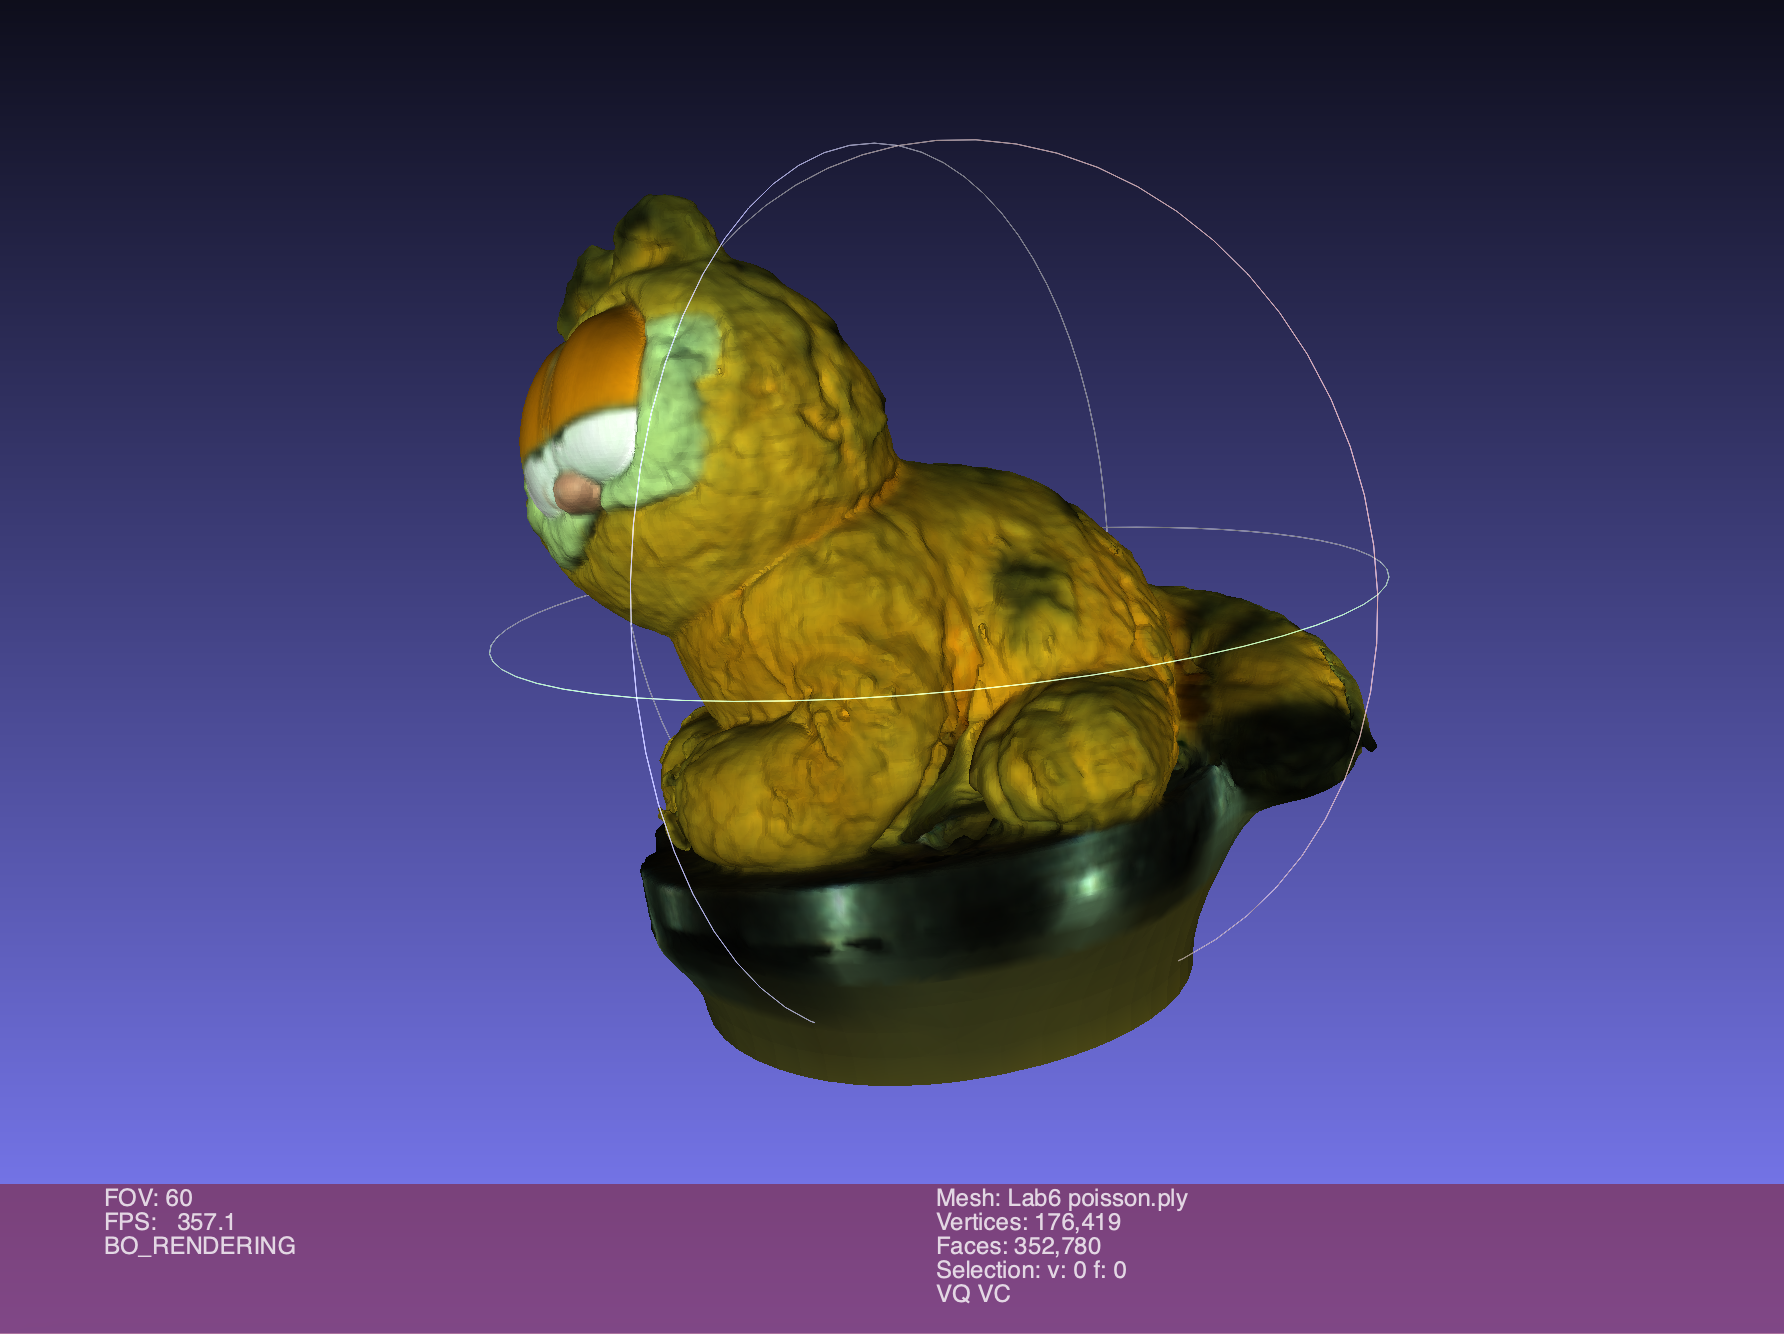
\includegraphics[width=0.8\textwidth]{screenshots/23.png}
			\caption{Konačan rezultat 2}
			\label{fig:yourlabel2}
		\end{figure}
		
		\begin{figure}[H]
			\centering
			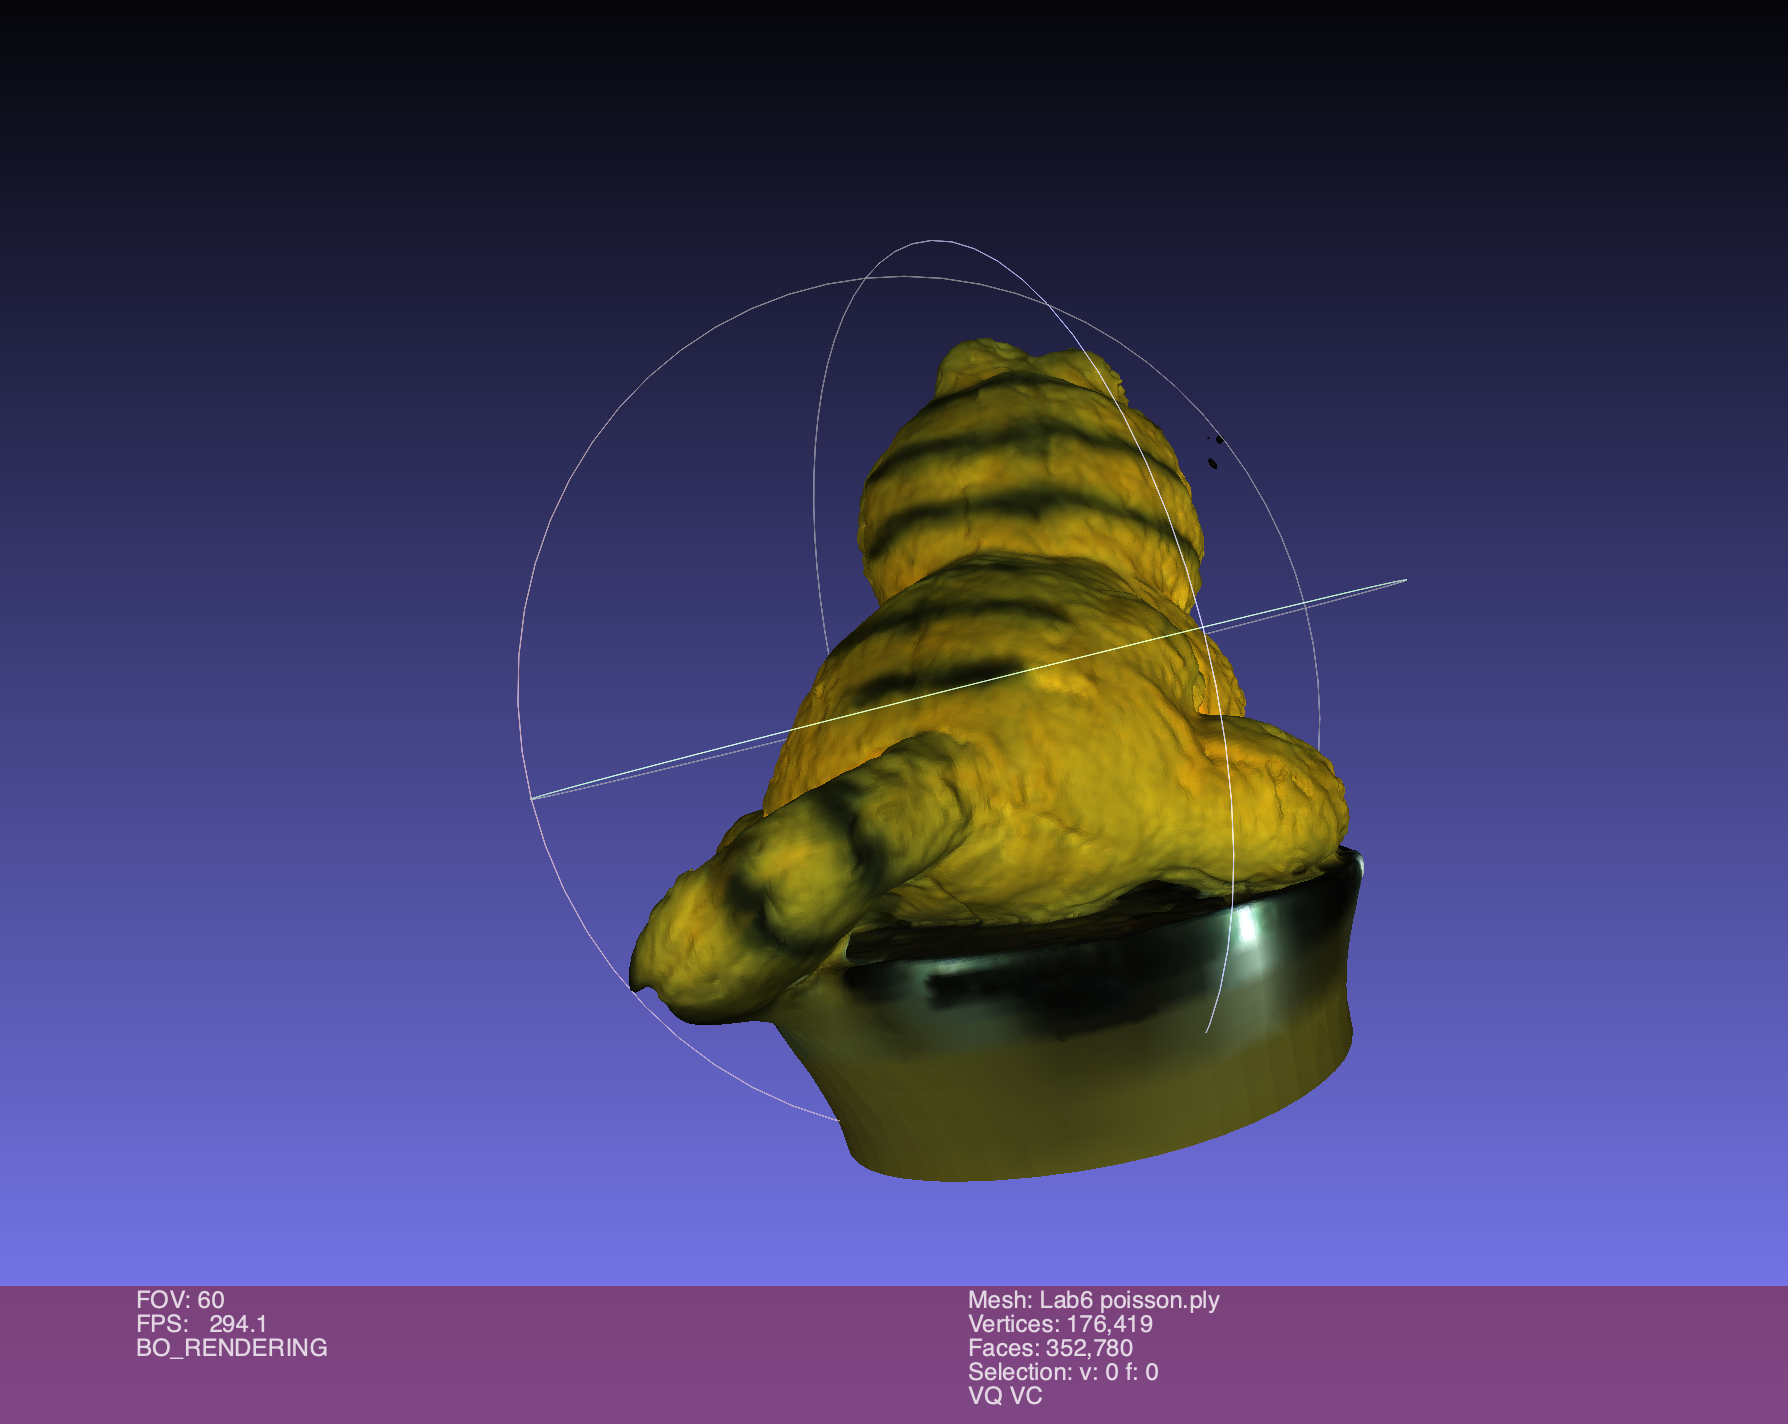
\includegraphics[width=0.8\textwidth]{screenshots/24.png}
			\caption{Konačan rezultat 3}
			\label{fig:yourlabel2}
		\end{figure}
		
		
		\begin{figure}[H]
			\centering
			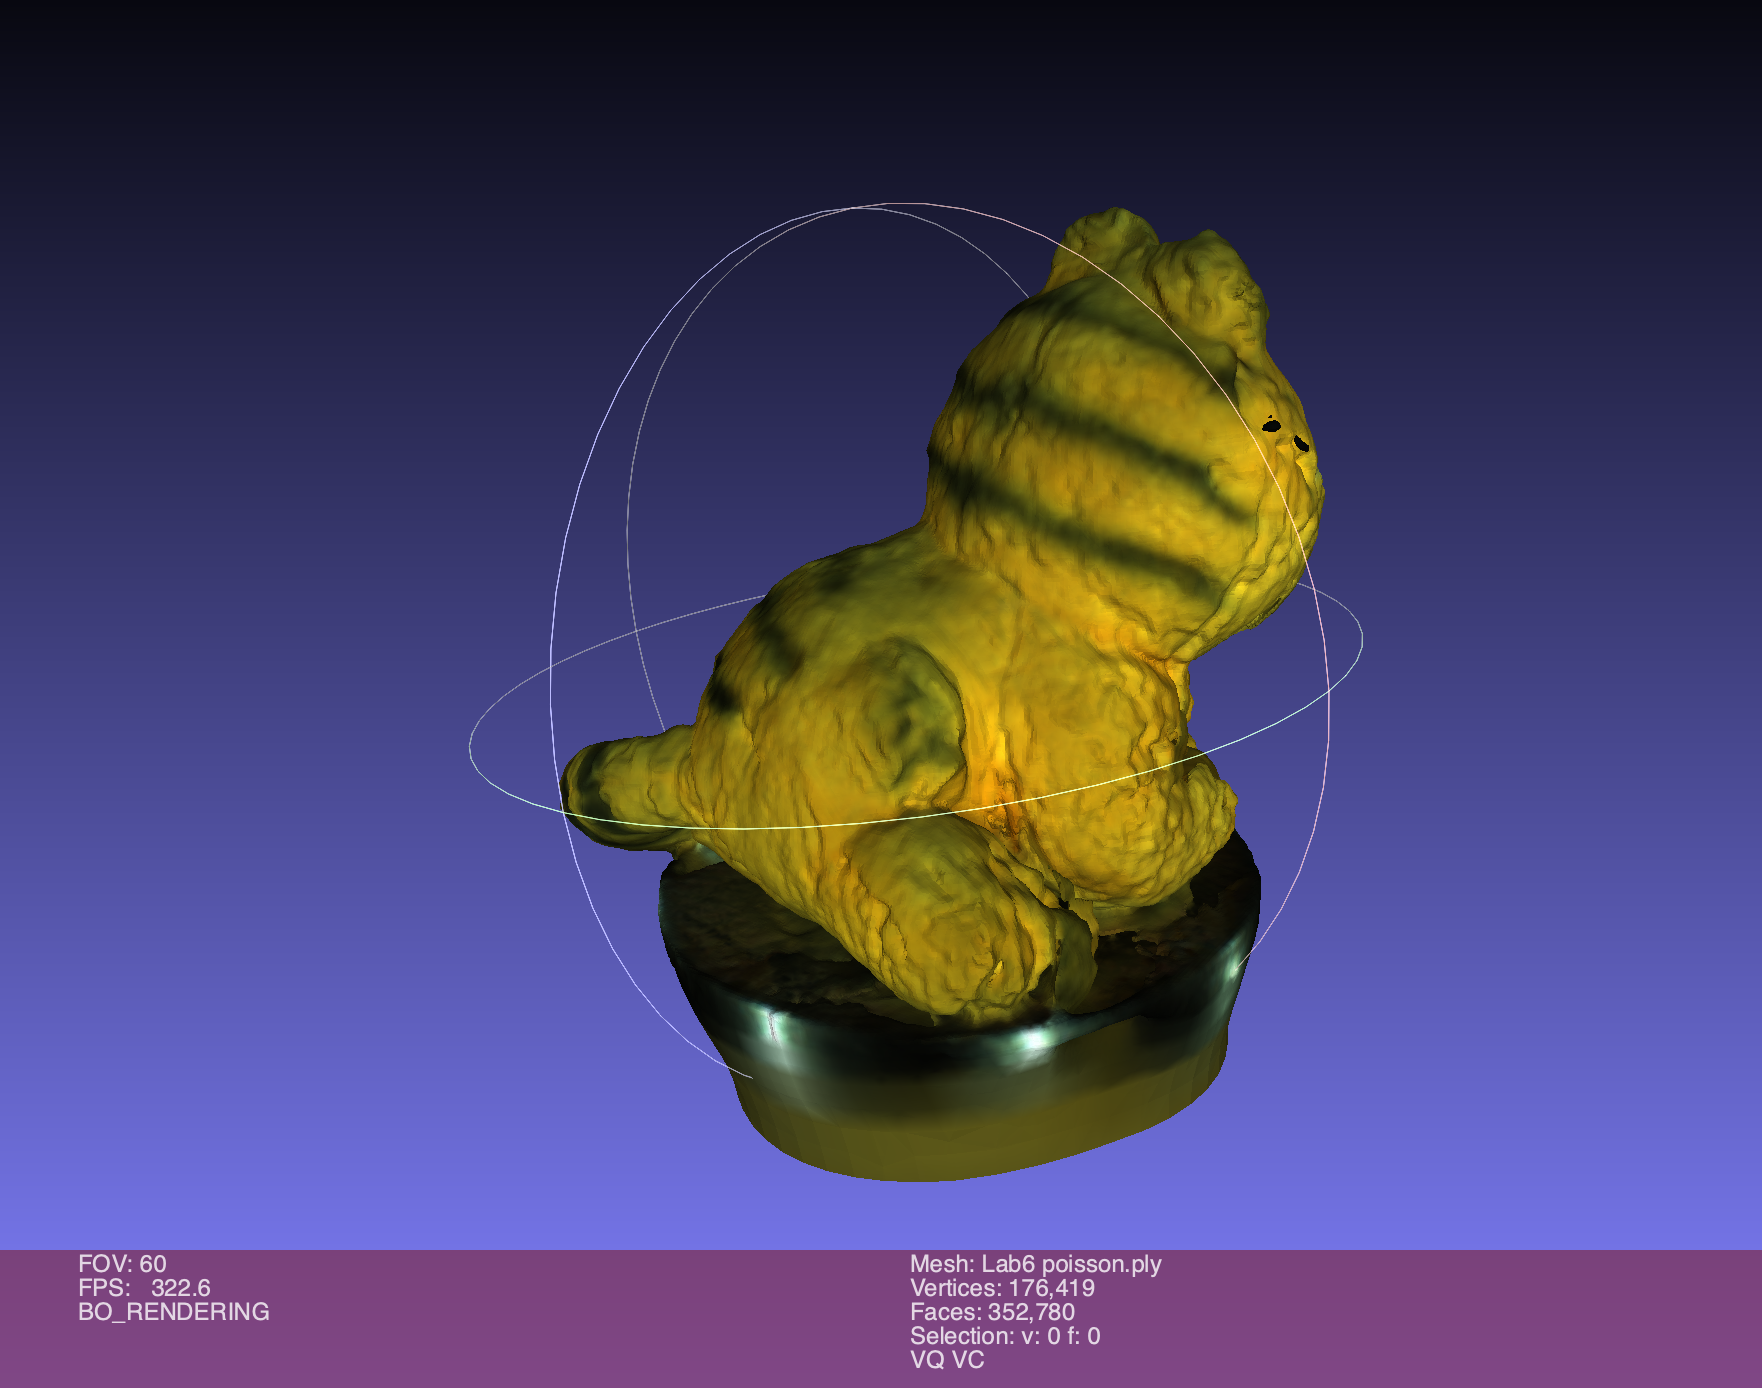
\includegraphics[width=0.8\textwidth]{screenshots/25.png}
			\caption{Konačan rezultat 4}
			\label{fig:yourlabel2}
		\end{figure}

	\eject
	
\end{document}
